\documentclass[]{article}

% Packages

% Pseudocode
\usepackage{algpseudocode}
\usepackage{algorithm}
\usepackage{arrayjob}

% Placing
\usepackage{float}
% Drawing
\usepackage{tikz}
\usetikzlibrary{arrows.meta,chains,%
	decorations.pathreplacing}
% Memory maps
\usepackage{bytefield}
% Simple trees
\usepackage{qtree}
% Better trees
\usepackage{forest} 
% Custom colors
\usepackage{xcolor}
% Comments
\usepackage{verbatim}
% math symbols
\usepackage{amssymb}
% csv reader
\usepackage{csvsimple}
% create file content
\usepackage{filecontents}
% Create c++ fields
\usepackage{listings}
% better tables
\usepackage{tabularx}
\usepackage{graphicx}
\usepackage{caption}
\usepackage{subcaption}
%control
\usepackage{ifthen}

% Plots
\usepackage{pgfplots}
\pgfplotsset{compat = newest}
\usepgfplotslibrary{fillbetween}
% cake diagrams
\usepackage{pgf-pie}  

% Better enumerate
\usepackage{outlines}

% snake lines
\usetikzlibrary{decorations.pathmorphing}
\tikzset{snake it/.style={decorate, decoration=snake}}

% Dependencies
\usepackage{mymacros}
\usepackage{parallelP}
\usepackage{cuda}

\lstset { %
    backgroundcolor=\color{black!5}, % set backgroundcolor
    basicstyle=\footnotesize,% basic font setting
    numbers=left,                    % where to put the line-numbers; possible values are (none, left, right)
    numbersep=5pt,                   % how far the line-numbers are from the code
    numberstyle=\tiny\color{black}, % the style that is used for the line-numbers
    rulecolor=\color{black},
    keywordstyle=\color{blue},
    tabsize=3,	
}


% Title
\title{Orthogonal Recursive Bisection on the GPU for Accelerated Load Balancing in Large N-Body Simulations \\ - \\ Bachelor Thesis}

\author{Andrin Rehmann}

% Start
\begin{document}

\maketitle

\newpage

\tableofcontents

\newpage
\section{Introduction}


The N-Body technique has been used for decades to simulate the Universe to compare theory with observations. It uses "particles" to represent objects of a certain mass and computes the forces by applying the gravity equation. As the forces operate over infinite distance it is necessary to consider all pair-wise interactions, making a naive implementation $\mathcal{O}(n^2)$. This does not scale with large particle counts.

A common solution is to partition the space, in which the particles are contained, into a set of subspaces, also called cells. These cells are then stored in a space partitioning tree data structure (SPTDS) in order to speed up the simulation with the Fast Multipole Method (FMM) to $O(n)$. 
Building the data structure uses a significant percentage of the overall simulation time. As of now this was usually done on the CPU, not leveraging GPU acceleration. 
In this thesis we establish upper limits for the speedup of GPU accelerated SPTDS building algorithms over its CPU only counterpart. We then propose, implement and compare efficient methods of building the SPTDS on the CPU and the GPU.

\TODO{Describe measurement results here}

\newpage
\section{Background}

Structures occurring within astrophysical simulations can be identified in real observed data\cite{Stadel2001}. Thus the simulations can help us understand the universe. Generated datasets with similar distributions to reality are used to seed the simulations. Mass field distribution are approximated with a large number of particles, where each of them represents a mass point. Numerical integration methods then compute the gravitational forces on each object.
Originally developed by Joachim Stadel during his PhD at University of Washington \cite{Stadel2001}, PKDGrav is a fully parallel N-Body code which is now maintained and improved by the ICS at UHZ \cite{ICS}. 
PkDGrav, as well as most state of the art simulation softwares, use a space partitioning tree data structure (SPTDS), which is used to partition a space into subspaces. Each cell (node), in the tree represents a subspace, and the children of the node represent the subspaces that are contained within the node's subspace. The mutlipole expansion is then applied to each cell of the SPTDS and the fast multipole method increases the runtime from $O(N^2)$ to $O(N)$ where $N$ is the total number of particles. \cite{Stadel2001}


\subsection{Fast Multipole Expansion} \label{sec:multipole}

In mathematics, a multipole is a concept used to approximate the shape of a physical body. In our case the body consists of the particles contained within the subspace, or volume of a cell. The multipole expansion is the mathematical series that results from this approximation. The resulting series can simplify the original body, by choosing a suitable precision.

To keep force integration within a reasonable error margin, in most cases it is not necessary to compute all $N$ to $N$ interactions. The fast multipole method can compute gravity in $O(N)$ runtime by leveraging the SPTDS. \cite{Stadel2001}

On a more intuitive level, one can imagine a large cluster of objects far away from planet Earth. If we wish to compute the interactions between every single object of the cluster and Earth, we will need to perform $O(N^2)$ computations. However, since the object is reasonably far away, it does not make sense to compute every interaction. Instead, we summarize the cluster into a single object and compute the gravity acting between planet Earth and the group. Consequently, objects within our own solar system would be too close to planet Earth to approximate its effects using a multipole. In such cases, it is necessary to perform all computations, however they can be hidden within a constant and do not affect the total runtime. 
Note that this example does not directly translate to the simulations, as a particle is not equivalent to a planet or a star. More on that in section \ref{sec:target-data}.


\subsubsection{Advantage of Cubic Bounding Volumes}\label{sec:cubic}

From \cite{Stadel2001}: "the opening radius of a cell is given by some constant factor times $r_{max}$". $r_{max}$ is the distance between the center of mass of a cell and its most distant corner. The opening radius correlates with the error ratio, which in turn influences how many timesteps have to be performed. Of the family of rectangular cuboids, the cube is the shape where the average distance between any point and its most distant corner point is the smallest. 

\subsection{ORB vs. K-d Trees}

A number of methods exist to create SPTDS, however since we require each cell on the same depth of the tree to encompass an almost equal number of particles method like octrees are not suitable. The k-d tree construction method however is strikingly similar to the ORB method we are using, however there is a slight difference in the construction process. 
The Orthogonal Recursive Bisection method constructs a SPTDS where all resulting cells represent subspaces, or volumes, similar to cubes. K-d construction methods generate SPTDS as well, but shapes of the resulting subspaces can be strongly skewed and are thus ill suited for FMM. Both algorithms start with a single cell and iteratively construct the SPTDS by searching for axis aligned planes cutting the volume of each leaf cell of the current SPTDS into two. From the resulting two volumes, two new cells are generated and appended to the SPTDS. 

In k-d tree construction, the axis lying orthogonal to the cut plane is chosen periodically, meaning all cells with an equal distance (depth) to the root of the SPTDS are cut with planes orthogonal to the same axis. In the case of ORB, the axis where a cells volume is largest is picked to compute an orthogonal plane. Therefore cells with the same depth can have cut planes of variable orientations. This make ORB special as it combines a balanced distribution with near cubic shapes.  

\subsection{Rise of the GPU}

Most if not all state of the art supercomputers are hybrid, meaning each node has a CPU as well as a GPU.\cite{TOP500} GPU accelerated code can increase the speed of many computations, where in most cases CUDA is used to fully leverage the hardware. 

The computational effort required in PKDGrav and most modern astrophysical N-Body simulations can be divided into three categories:

\begin{enumerate}
	\item \textbf{Global Tree Building / Load Balancing:} In supercomputers, particles are distributed equally among computing nodes to leverage node level parallelization. ORB is used to generate a well suited SPTDS for FMM on a node level.
	\item \textbf{Local Tree Building:} The same approach is repeated on a local level, where instead of distributing the workload among nodes, its distributed among threads. The tree from step 1. is expanded by the locally computed tree.
	\item \textbf{Force Calculation and Integration:} The STPDS constructed in step 1. and 2. combined with FMM is used to compute force integration. 
\end{enumerate}

In PKDG each category is about one third of the total calculation time\cite{Stadel2001}. Making Global (1.) and Local Tree Building (2.) subjects to possible performance improvements, as GPU acceleration is as of now only exploited in Force Calculation and Integration(3.).

Our main objective is to improve the runtime of astrophysical simulations, or more specifically PKDGrav. Simultaneously penalties with regards to $N$, the total number of particles, should be kept as low as possible. Simulation accuracy benefits from large $N$ as well as an increased number of time steps. As GPU accelerations act on a low level, hardware specific details are relevant. We want do adapt and optimize the algorithms with regards to the target computer Piz Daint.


\subsection{Related Work}


A number of GPU accelerated k-d tree construction algorithms exists, however the methods cannot simply be translated to ORB due to different axis choosing method. Fore example in the master thesis of Voglsam \cite{rrt} a k-d tree is computed on the GPU and used to improve ray tracing for 3D graphics. However it makes use of a binning algorithm to find an optimal cut across cells of the same depth, which can be done in a single iteration. However in our case the axes for cells of the same depth vary.

When we subdivide ORB into its individual components as shown below, some subroutines can be computed using fairly general algorithms, which have already been implemented and optimized for the GPU in many open source libraries. 

\begin{outline}[enumerate]
	\1 Cut cells on last level in tree
	\2 Make cut plane position guess
	\2 Count number of particles left to the cut plane
	\2 Repeat 1. till correct plane was found
	\1 Partition particles
	\1 Repeat till desired depth was reached
\end{outline}

Thrust by \textit{NVIDIA} \cite{thrust} has an implementation of a reduction, which can be used to perform step 1.b), a binary search is equivalent to the entire step 1. and finally it also exposes a partition interface. The library is very high level and does not allow us to control memory operations, which are very crucial to a highly efficient implementation of ORB. 
Furthermore CUB \cite{cub}, also developed by \textit{NVIDIA}, exposes a more low level API of the equivalent elements but the implementation is not general enough to deal with some critical performance issues. As the SPTDS grows, so do the number of leaf cells and thus the number of cells for which a cut plane has to be found in the same iteration. If we initialize a kernel for each cell, the number of kernels initialized grow exponentially, resulting in kernel invocation overheads dominating the actual computational costs.


\newpage


%After the SPTDS is built, we compute the multipole for all cells in the tree. This allows us to dynamically select more or less detailed functions to represent a group of particles. Depending on the distance between the particle we want to determine the forces for and the particles which exert the forces, we might choose a higher or lower multipole expansion.

\begin{comment}
\subsection{Procedure Overview}

When a simulation is initialized, all data is distributed randomly among the nodes. With regards to particle positions, the target data is initially unstructured, therefore we have no way distribute the particles in a better way. As we want to leverage FMM we need to compute a SPTDS across all nodes. 

The SPTDS has to be recomputed each time after force integration is computed.  Some particles may have crossed their cell boundaries during the process, violating the very constraint that all particles "owned" by a cell are contained within its volume. There are smarter ways to update the tree, which include more relaxed constraints, we will not focus on updating strategies and simply recompute the entire tree after each time step.

Depicted below is an illustration giving a high level overview over the necessary steps required to perform the load balancing. 

\begin{enumerate}
	\item 
	The simulation data is generated and located on a central storage device.
	
	\pgfmathsetseed{10}
	\begin{figure}[H]
		\begin{center}
			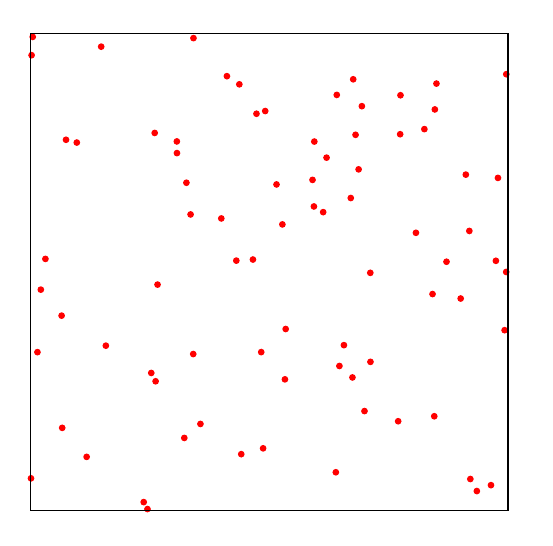
\begin{tikzpicture}
				\foreach \i in {1,...,80}{
					\filldraw [red] (rnd*\linewidth*0.5,rnd*\linewidth*0.5) circle (1pt) node [anchor=west]{};
				}
				\draw (0,0) rectangle (\linewidth*0.5, \linewidth*0.5);
			\end{tikzpicture}
		\end{center}
		\caption{Initial data with particles}
	\end{figure}
	\item
	Since the data is initially unstructured, is is distributed randomly among the nodes in the super computer.
	\pgfmathsetseed{10}
	\begin{figure}[H]
		\begin{center}
			\foreach \j in {1,...,4}{
				\begin{minipage}[c]{0.2\linewidth}
					\begin{tikzpicture}
						\foreach \i in {1,...,20}{
							\filldraw [red] (rnd*\linewidth,rnd*\linewidth) circle (1pt) node [anchor=west]{};
						}
						\draw (0,0) rectangle (\linewidth, \linewidth);
					\end{tikzpicture}
				\end{minipage}
			}
		\end{center}
		\caption{Particles are randomly distributed among 4 nodes}
	\end{figure}
	\item
	 The SPTDS is constructed with ORB. The tree is computed globally across all nodes, meaning the volumes of the individual cell are identical for all nodes.
	\pgfmathsetseed{10}
	\begin{figure}[H]
		\begin{center}
			\foreach \j in {1,...,4}{
				\begin{minipage}[c]{0.2\linewidth}
					\begin{tikzpicture}
						\foreach \i in {1,...,20}{
							\filldraw [red] (rnd*\linewidth,rnd*\linewidth) circle (1pt) node [anchor=west]{};
						}
						\draw (0,0) rectangle (\linewidth, \linewidth);
						
						\draw (0,0) rectangle (\linewidth*0.55, \linewidth);
						
						\draw (0,0) rectangle (\linewidth*0.55, \linewidth*0.6);
						
						\draw (\linewidth*0.55,0) rectangle (\linewidth, \linewidth*0.5);
						
					\end{tikzpicture}
				\end{minipage}
			}
		\end{center}
		\caption{Space partitioning tree data structure is computed}
	\end{figure}
	
	\item
	In a final step the particles are redistributed among the nodes, such that each node stores all particles contained in the volume of a unique cell.
	\begin{figure}[H]
		\begin{center}
			\pgfmathsetseed{10}
			\begin{minipage}[c]{0.2\linewidth}
				\begin{tikzpicture}
					\foreach \i in {1,...,80}{
						\filldraw [red] (rnd*\linewidth,rnd*\linewidth) circle (1pt) node [anchor=west]{};
					}
					\draw[fill=white] (0,0) rectangle (\linewidth*0.55,  \linewidth*0.6);
					\draw[fill=white] (\linewidth*0.55,0) rectangle (\linewidth,  \linewidth*0.5);
					\draw[fill=white] (0,\linewidth*0.6) rectangle (\linewidth*0.55,  \linewidth);
					\draw (\linewidth*0.55,\linewidth*0.5) rectangle (\linewidth,  \linewidth);
					
				\end{tikzpicture}
			\end{minipage}
			\pgfmathsetseed{10}
			\begin{minipage}[c]{0.2\linewidth}
				\begin{tikzpicture}
					\foreach \i in {1,...,80}{
						\filldraw [red] (rnd*\linewidth,rnd*\linewidth) circle (1pt) node [anchor=west]{};
					}
					\draw[fill=white] (0,0) rectangle (\linewidth*0.55,  \linewidth*0.6);
					\draw[fill=white] (\linewidth*0.55,0) rectangle (\linewidth,  \linewidth*0.5);
					\draw (0,\linewidth*0.6) rectangle (\linewidth*0.55,  \linewidth);
					\draw[fill=white] (\linewidth*0.55,\linewidth*0.5) rectangle (\linewidth,  \linewidth);
					
				\end{tikzpicture}
			\end{minipage}
			\pgfmathsetseed{10}
			\begin{minipage}[c]{0.2\linewidth}
				\begin{tikzpicture}
					\foreach \i in {1,...,80}{
						\filldraw [red] (rnd*\linewidth,rnd*\linewidth) circle (1pt) node [anchor=west]{};
					}
					\draw[fill=white] (0,0) rectangle (\linewidth*0.55,  \linewidth*0.6);
					\draw (\linewidth*0.55,0) rectangle (\linewidth,  \linewidth*0.5);
					\draw[fill=white] (0,\linewidth*0.6) rectangle (\linewidth*0.55,  \linewidth);
					\draw[fill=white] (\linewidth*0.55,\linewidth*0.5) rectangle (\linewidth,  \linewidth);
				\end{tikzpicture}
			\end{minipage}	
			\pgfmathsetseed{10}
			\begin{minipage}[c]{0.2\linewidth}
				\begin{tikzpicture}
					\foreach \i in {1,...,80}{
						\filldraw [red] (rnd*\linewidth,rnd*\linewidth) circle (1pt) node [anchor=west]{};
					}
					\draw (0,0) rectangle (\linewidth*0.55,  \linewidth*0.6);
					\draw[fill=white] (\linewidth*0.55,0) rectangle (\linewidth,  \linewidth*0.5);
					\draw[fill=white] (0,\linewidth*0.6) rectangle (\linewidth*0.55,  \linewidth);
					\draw[fill=white] (\linewidth*0.55,\linewidth*0.5) rectangle (\linewidth,  \linewidth);
				\end{tikzpicture}
			\end{minipage}
		\end{center}
		\caption{Leaf cells of data structure are distributed among nodes}
	\end{figure}
\end{enumerate}
\end{comment}


\newpage
\section{Orthogonal Recursive Bisection (ORB)} \label{section:orb}


%https://de.overleaf.com/learn/latex/TikZ_package
%https://texample.net/tikz/examples/
Each cell in the SPTDS is enriched with the following properties:

\begin{itemize}
	\item \textbf{$V_{cell}$} 3D volume where all corresponding particles are contained within.
	\item \textbf{$d_{cell}$} Number of leaf cells to be found among all subsequent cells.
	\item \textbf{$N_{cell}$} Number of particles encompasses in the volume of the cell. 
\end{itemize}

Naturally each cell has two pointers pointing to its two children, which are used to traverse the tree, parent cell pointers important but could be added as well.


\subsection{Target Data and Notation}\label{sec:target-data}

\begin{comment}
The target data consists of $N$ particles where we use the following notations:

constrained realization
Gaussian random distribution, modified to match the measured power.

The higher the resolution the more accurate the result.

Large scales are more uniform, small scale 

smallest thing you want to be able to resolve. 

boxes around a giga parsec

want to be able to resolve galaxies, milky way 10^12 solar masses,

want to be able to resolve smaller galaxies, 10^8 for a single particle
Imp 
\end{comment}
A modified random Gaussian distributed is used to generate the target dataset, where its set to fit measured constraints of the actual universe. Thus the number of particles can set dynamically. In the simulation, a single particle has a mass of $10^8$ solar masses. 


\begin{itemize}
	\item We define the space of binary numbers with a precision of $p$ as $\mathbb{B}_p$ where we have $a \in \mathbb{B}_p \Leftrightarrow a \in \{0,1\}^{p}$
	\item We define the corner coordinates of root domain with $\vec{lower}, \vec{upper}$ where we have $\vec{lower}, \vec{upper} \in \mathbb{B}_p^3$. 
	\item We define the coordinates of a particle $i$ as $\vec{x_i}$ for which holds $\{\vec{x} | \vec{lower} \leq \vec{x} \leq \vec{upper}, \vec{x} \in \mathbb{B}_p^3 \}$.
	When refering to a single coordinate of a particle object we do so by writing $\vec{x}_{i,j}$. Finally the array of all particles positions in a single axis is denoted as $\vec{x}_{:,j}$. 
	
\end{itemize}

It lies in the nature of the universe, that large clusters of particles are found in some places, whereas other areas may be vastly empty of any objects. This is a very crucial characterization and differentiates this dataset from many other application of FMM, where the distribution are more uniform.

\begin{figure}[H]
	\begin{center}
		\begin{tikzpicture}
			\randistr{10}{5}{100}
			\draw (0,0) rectangle (10, 5);
			\filldraw  (0,0) circle (3pt) node [anchor=west]{};
			\node[yshift=-0.3cm, xshift=-0.3cm] at (0,0) {$lower$};
			
			\filldraw  (10,5) circle (3pt) node [anchor=west]{};
			\node[yshift=0.3cm, xshift=-0.3cm] at (10,5) {$upper$};
		\end{tikzpicture}
	\end{center}
	\caption{Uniform random distribution of 3D coordinates in cube domain projected onto a 2d plane}
\end{figure}


\subsection{Memory and Workload Balancing}\label{balancing}
As mentioned we want to (1) improve the runtime of ORB whilst (2) at the same time keeping the number of particles $N$ as large as possible. There exists some averse effects when disregarding interactions between minimizing runtime and maximizing $N$.

To reduce the force integration error across all particles, some particles require more timesteps than others. This is caused by the vastly variant forces which are exerted on the particles. Whilst some follow a straight path with an almost constant velocity requiring little computational effort for great precision, others are influenced by strong gravitational poles resulting in highly curved movement paths and correlating with higher numbers of timesteps required.

We denote the workload for a particle $p_i$ as the weighting function $w(p_i)$. The workload correlates with the number of simulations steps, that need to be computed for a single particle. In an optimally parallelized system balanced in terms of computational effort, the workload should be very similar among computing units. Where ideally the sum over all the particles considered by a thread is equal to the sum of all others. With strongly varying weights among particles, perfectly balancing the computational effort, results in a unbalanced distribution in terms of memory. 

Let us consider a simple example to illustrate the point. Given the set of particles $A = \{p_1, p_2, .., p_{2m/3}\}$ and respectively $B = \{p_{2m/3 + 1}, p_2, .., p_{m}\}$. This yields a total number of particles equivalent to $N = m$. We assuming that $\forall p \in A : w(p) = 1$ and $\forall p \in B : w(p) = 2$. 
We assign all particles from set $A$ to process with rank 0 and the particles from B to rank 1. It follows $\sum_{p\in A} w(p) = \sum_{p\in B} w(p)$. Thus the two processors are balanced in terms of computing costs, but not in terms of memory size. In fact, process with rank 0 has $2m/3$ elements and rank 1 has $m/3$ elements. Assuming each process has a memory size of $2m/3$, then clearly this configuration is not optimal. If we were to favor memory balancing, we could assign $2m/3$ to each processor and we would be able process $(4/3) \times m$ particles in total, which is larger than the original $N$ and therefore favorable since a dataset with a larger $N$ could be used.

To which degree its ideal favor memory over workload balancing is difficult to answer. For now parametrize the workload using the weighting function. If we decide to completely ignore the workload balancing and solely focus on memory balancing, we can simply set $w(p_i) = 1$ for all particles.

\subsection{ORB}


To introduce the ORB algorithm, we consider a recursive implementation of ORB as it is easier to understand than the iterative version. We define all cell properties recursively, allowing us to describe the algorithm in detail and derive the necessary constraints.

As we initialize the recursion with the root cell alone, it follows that $V_{root}$ is equivalent to entire volume of the input data. $d_{cell} = d$ and $N_{root} = N$ are true per definition of $N$ and $d$. 
When a cell is cut into two child cells, we refer to the children as $leftCell$ and $rightCell$. For any cell the following equations hold:

\begin{center}
	\begin{equation}
		depth_{cell} = \lceil \log_2{d_{cell}} \rceil 
	\end{equation}
\end{center}

\begin{center}
	\begin{equation}\label{eq:v}
		V_{cell} = V_{leftCell} \cup V_{rightCell}
	\end{equation}
\end{center}

\begin{center}
	\begin{equation}\label{eq:v2}
		V_{leftCell} \cap V_{rightCell} = \emptyset
	\end{equation}
\end{center}

Defining $d_{cell}$ for each cell is especially important, since we want to ensure the final tree is a nearly complete binary tree. The way we define $d_{leftCell}$ and $d_{rightCell}$ we ensure that on the last level of tree the cells are filled from the left to the right. This way no gaps are present and the tree can be stored as a heap in an array. 

\begin{center}
	\begin{equation} \label{eq:d1}
		d_{leftCell} = \min \{ d_{cell} - 2^{depth_{cell} -2}, 2^{depth_{cell} - 1}\}
	\end{equation}
\end{center}

\begin{center}
	\begin{equation}  \label{eq:d2}
		d_{rightCell} = \max \{ d_{cell} - 2^{depth_{cell} -1}, 2^{depth_{cell} - 2}\}
	\end{equation}
\end{center}

Finally the number of particles encompassed in $V_{leftCell}$ and $V_{rigtCell}$ are defined as follows:

\begin{center}
	\begin{equation}\label{eq:N1}
		N_{leftCell} = min \left \{ x \in \{0,...,N_{cell} \} : \sum_{i=0}^{x} w(p_i) \geq \frac{d_{leftCell}}{d_{cell}} \times \sum_{i=0}^{N_{cell}} w(p_i) \right \} - 1
	\end{equation}
\end{center}

\begin{center}
	\begin{equation}\label{eq:N2}
		N_{rightCell} = N_{cell} - N_{leftCell}
	\end{equation}
\end{center}

To simplify the visual and numeric explanation of the ORB algorithm, we assume $\forall i \in \{0,..,N\} : w(p_i) = 1$.

The cut plane, which divides $V_{leftCell}$ and $V_{rightCell}$ is axis aligned an thus orthogonal to a given axis $a$. Thus searching for a single value $c$ is sufficient to construct the plane, where $c$ is the position of the plane along the axis $a$. The plane is considered ideal if the number of particles where $x_{i,a} \leq c$ are equivalent to $N_{leftCell}$. 

After a plane is found, we can divide or cut the $V_{cell}$ in two volumes, where $V_{leftCell}$ and $V_{rightCell}$ are constrained by the original $V_{cell}$ and the cut plane. As defined in equation \ref{eq:v2} the volumes do not intersect, thus $V_{leftCell}$ along axis $a$ ends at $c$, where $V_{rightCell}$ start at $c$.
    
  
\subsubsection{Algorithm}

Algorithm \ref{proc:orbmain} as mentioned below, is the main routine of ORB. All the volumes are described using a lower and an upper boundary point, sufficiently describing a box, thus the only input parameters required is $x$ storing the particles positions, $lower$, $upper$ and finally $d$.
If $d$ is equal to 1, this means the reduction must not be continued, as the target of a single subsequent leaf cell is already reached, since the cell itself is treated as a leaf cell. The stopping condition is formulated on lines 2-4. 
Line 6 describes a call to a method called $maxIndex()$, which essentially compares all provided values and returns the index of the maximum values. The result $i$ provides us with the axis where the cell volume is largest. 
$d_{leftCell}$ is computed as described in equation \ref{eq:d1} and its results is stored in a variable named $d^\prime$. All prerequisites are met to compute the actual cut with the $cut$ method which we will explain in more detail in section \ref{sec:root}. The return value stored in $cut$ is equivalent to the position of the cut plane along the cut axis. Using the $cut$ value, the array of particles is partitioned as described in \ref{sec:part} returning the $mid$ value which is the pivot index of the partitioning.
Finally we can divide the original volume into two volumes as described on lines 10-13 and recursively call $ORB$ method where we provide it with two slices of the $x$ array.

\begin{algorithm}[H]
 	\begin{algorithmic}[1]
 		\Procedure{orb}{$x$, $\vec{lower}, \vec{upper}, d$}
 		\If{d = 1}
 		\State \Return	\Comment{Stopping condition}	
 		\EndIf
 		\State $\vec{size} = \vec{upper} - \vec{lower}$
 		\State $i = maxIndex(\vec{size}_0, \vec{size}_1, \vec{size}_2)$ \Comment{Get index of max value}
 		\newline
 		\State $l = \lceil \log_2{d} \rceil$ \Comment{Depth}
 		\State $d^\prime = \min \{ d - 2^{l -2}, 2^{l - 1}\}$
 		
 		\State $cut = cut(x, \vec{lower}_{i}, \vec{upper}_{i}, i, \frac{d^\prime}{d} )$\Comment{Find cut plane}
 		\State $mid = partition(x, split, axis)$ \Comment{Partition particles}
 		\newline
 		
 		\State $\vec{upper^\prime} = \vec{upper}$
 		\State $upperChild_{i} = cut$
 		\State $\vec{lower^\prime} = \vec{lower}$
 		\State $lowerChild_{i} = cut$
 		\newline
 		
 		\State \Call{orb}{$x_{0:mid,:}$,$\vec{lower}, \vec{upper^\prime}, d^\prime $} 
 		\State \Call{orb}{$x_{mid:len(x),:}$$\vec{lower^\prime}, \vec{upper}, d - d^\prime $}
 		\EndProcedure
 	\end{algorithmic}
 	\caption{The ORB main routine}\label{proc:orbmain}
\end{algorithm}



\subsection{By Example}

A sample dataset is proposed to help with visual and numerical explanations of the algorithm. All particles in the sample dataset are assumed to have a weight of 1.

\begin{filecontents*}{particles10.csv}
	x,y,id,o1,o2,x2,y2
	0.4,0.3,0,0,0,0.4,0.3
	0.2,0.6,1,2,1,0.2,0.6
	0.8,0.9,2,1,2,0.9,0.8
	0.6,0.5,3,0,0,0.6,0.5
	0.3,0.8,4,1,1,0.3,0.8
	0.7,0.1,5,2,2,0.7,0.1
	0.9,0.3,6,2,2,0.9,0.3
\end{filecontents*}

\begin{filecontents*}{particles11.csv}
	x,y,id
	0.4,0.3,0
	0.2,0.6,1
	0.3,0.8,4
	0.6,0.5,3
	0.8,0.9,2
	0.7,0.1,5
	0.9,0.3,6
\end{filecontents*}


\begin{filecontents*}{particles12.csv}
	x,y,id
	0.4,0.3,0
	0.6,0.5,3
	0.3,0.8,4
	0.2,0.6,1
	0.8,0.9,2
	0.7,0.1,5
	0.9,0.3,6
\end{filecontents*}

We explore the algorithm visually using the provided example dataset:


\begin{figure}[H]
	\begin{center}
		\begin{minipage}[c]{0.2\linewidth}
			\csvreader[
			tabular=ccc,
			table head=\hline \bfseries{x} & \bfseries{y} & \bfseries{id} \\\hline,
			late after last line=\\\hline % horizontal line at the end of the table
			]{particles10.csv}{}{\csvcoli & \csvcolii & \csvcoliii}
		\end{minipage}
		\begin{minipage}[c]{0.7\linewidth}
			\begin{tikzpicture}
				\begin{axis}
					[
					nodes near coords,
					xmin=0,
					xmax=1,
					ymin=0,
					ymax=1
					]
					\addplot+[
					only marks,
					point meta=explicit symbolic
					] table [
					x=x, 
					y=y, 
					meta=id, 
					col sep=comma] 
					{particles10.csv};
				\end{axis}
				
			\end{tikzpicture}
		\end{minipage}
	\end{center}
	\caption{Example distribution with $N$ = 7}
\end{figure}

\begin{figure}[H]
	
	\centering
	\begin{tikzpicture}
		\begin{axis}
			[
			nodes near coords,
			xmin=-0.,
			xmax=1.,
			ymin=-0.,
			ymax=1.,
			]
			\addplot    +[
			only marks,
			point meta=explicit symbolic
			] table [
			x=x, 
			y=y, 
			meta=id, 
			col sep=comma] 
			{particles10.csv};
			\draw [fill=red!20](0.0,0.0) rectangle (1, 1);
			\node[below] at (0.5, 1){$cell_1$};
		\end{axis}
	\end{tikzpicture}
	\caption{Example particles with ORB at recursion depth 0}
	\label{fig:orb1}
\end{figure}

\begin{figure}[H]
	\centering
	\begin{forest}
		[$cell_1$
		[]  
		]
	\end{forest}    
	\caption{Tree with ORB at recursion depth 0}
	\label{fig:orb11}
\end{figure}

Depicted in figure \ref{fig:orb1} \&  \ref{fig:orb11} is the SPTDS after initialization: there is only one $cell_1$ which is root and $V_{cell_1}$ encompasses the entire domain which in this case is the rectangle ranging from 0 to 1 in both the x and y axis. $d_{cell_1}$ is equivalent to 3 and $N_{cell_1}$ is 7. 

\begin{figure}[H]
	\begin{center}
		\begin{tikzpicture}
			\pgfmathsetseed{2};
			\begin{axis}
				[
				nodes near coords,
				xmin=-0.,
				xmax=1.,
				ymin=-0.,
				ymax=1.,
				]
				\addplot+[
				only marks,
				point meta=explicit symbolic
				] table [
				x=x, 
				y=y, 
				meta=id, 
				col sep=comma] 
				{particles10.csv};
				\draw [fill=green!20](0.0,0.0) rectangle (0.65, 1);
				\draw [fill=blue!20](0.65,0.0) rectangle (1, 1);
				\node[below] at (0.2, 1){$cell_2$};
				\node[below] at (0.7, 1){$cell_3$};
			\end{axis}
			
		\end{tikzpicture}
	\end{center}
	\caption{Example particles with ORB at recursion depth 1}
	\label{fig:orb2}
\end{figure}

\begin{figure}[H]
	\centering
	\begin{forest}
		[$cell_1$
		[$cell_2$][$cell_3$]  
		]
	\end{forest}    
	\caption{Tree with ORB at recursion depth 1}
	\label{fig:orb22}
\end{figure}
A cut plane, which translates to a cut line in our simplified 2D example is constructed and $cell_2$ and $cell_3$ are generated accordingly.

\ref{fig:orb2} \&  \ref{fig:orb22} Depict a SPTDS of depth 2, or two levels, where a cut plane was found dividing $V_{cell_1}$ into $V_{cell_2}$ and $V_{cell_3}$, $d_{cell_2} = 2$ and $d_{cell_3} = 1$ subsequently are calculated, meaning $cell_3$ is considered a leaf cell. Thus we can compute $N_{cell_2}$ using a simplified version of equation \ref{eq:N1} since we assume all weights are equal 1: $N_{cell_2} = \lfloor \frac{d_{cell_2}}{d_{cell_3}} * N_{cell_1} \rfloor = \lfloor \frac{2}{3}  * 7 \rfloor = 4$ subsequently $N_{cell_3} = 3$. 

\begin{figure}[H]
	\begin{center}
		\begin{tikzpicture}
			\pgfmathsetseed{2};
			\begin{axis}
				[
				nodes near coords,
				xmin=-0.,
				xmax=1.,
				ymin=-0.,
				ymax=1.,
				title=Recursion depth 2
				]
				\addplot+[
				only marks,
				point meta=explicit symbolic
				] table [
				x=x, 
				y=y, 
				meta=id, 
				col sep=comma] 
				{particles10.csv};
				\draw [fill=pink!20](0.0,0.0) rectangle (0.65, 0.55);
				\draw [fill=yellow!20](0.0,0.55) rectangle (0.65, 1);
				\draw [fill=blue!20](0.65,0.0) rectangle (1, 1);
				\node[below] at (0.2, 1){$cell_4$};
				\node[above] at (0.2, 0){$cell_5$};
				\node[below] at (0.7, 1){$cell_3$};
			\end{axis}
			
		\end{tikzpicture}
	\end{center}
	\caption{Example particles with ORB at recursion depth 2}
	\label{fig:orb3}
\end{figure}

\begin{figure}[H]
	\centering
	\begin{forest}
		[$cell_1$
		[$cell_2$ [$cell_4$] [$cell_5$]][$cell_3$]  
		]
	\end{forest}
	\caption{Tree with ORB at recursion depth 2}
\end{figure}

Again the procedure is repeated for $cell_2$ but not for $cell_3$ as there recursion is terminated by the stopping condition. Finally we end up with $cell_4$ and $cell_5$ where the stopping condition is met as well. The resulting SPTDS has 3 leaf cells and partitions the space into three subspaces.

%Since $d_{cellLeft} - d_{cellRight}$ must always be $\leq 1$, it must hold that the tree is a nearly complete binary tree. Therefore we can conclude that the height of the tree is equal to $\lceil log(d) \rceil$ and the total number of nodes (not only leaf nodes) is $log(d) \times d$. Since we have a nearly complete binary tree, we also have the possibility of storing it as a heap\cite{algorithms} data-structure in an array.  This increase the performance of many tree operations, since we will not have to perform a tree walk to access individual cells in the tree. Furthermore child an parent cells can be accessed without pointers but directly by computing their index in the array.


\subsection{Root finding} \label{sec:root}


%Finding the median of a large particle array is an essential step for ORB. We will thus explore different algorithms alongside their advantages and disadvantages for our specific use case.
%Note that there exists approximation algorithms for example the median of medians algorithms. But the correctness guarantee of the median lying between 30\% and 70\% is not good enough in our case. If we were to implement such an approximation algorithms we would run into similar issues as described in \ref{sec:balancing}. But in this case the unequal memory balancing do not have the advantage of equal workload balancing, which in turn will worsen the performance and the maximum number of workable particles. Thus we will only consider approximation algorithms, if their approximation to the ideal values are very exact and can be determined.


The $cut$ algorithm takes an array of particle positions $x$, an $axis$, $left$ and $right$ boundaries and a $percentage$. Its goal is to return a position along the cut axis such that the particles less or equal to the a $cut$ value are equivalent to the percentage multiplied by the length of the $x$ array.

The problem is related to a selection algorithm and a quick select\cite{algorithms} could be used. However quick select has a worst case runtime of $O(n^2)$. Furthermore median algorithms could be explored as well, but they are mostly approximation algorithms with bad worst case runtimes. We can reformulate the problem as a root finding problem. To do so we define a function $f(c)$ which evaluates the number of elements smaller than the cut value minus half the number of total particles. When the function evaluates to zero, we have found an axis aligned cut plane, where exactly half the particles are located on the left side. There exist many different solvers for the root-finding problem, but the most stable and easiest to implement is the bisection method. Some solver combine approximate solver with the stable bisection method to generate fast but stable root finding methods. Such algorithms could be explored in later work.

Since we are operating on binary numbers with a limited precision, the bisection method is guaranteed to terminate after $p$ steps.

\subsubsection{Bisection Method}

Initially an estimation for a cut is made, in this case the exact middle of the domain boundaries. Some median finding algorithms use improved guessing to speed up the process, again a method which could be leveraged in later work. 

Because the maximal number of iterations is known, a loop can be used as seen below in algorithm \ref{proc:cut} on line 4. A cut is then computed (line 5), which in the first iteration is the center position between left and right. We then check weather the stopping condition has already been reached (line 7-9), meaning the cut lies within $\alpha$ points of the ideal result. If it was not reached the boundaries can be improved as follows: In case there are too many elements left of the cut, we know that the cut position was chosen too far to the right and we can be sure that the ideal cut must be left of the current guess. Therefore we adjust the boundaries, in this case we set $righ$ equal to $cut$ as seen on line 13. The analog concept can be applied in the other case (line 11). 

\begin{algorithm}[H]
		\begin{algorithmic}[1]
			\Procedure{cut}{$x, left, right, axis, percentage$}
			\State $nLeft = 0$
			\State $cut = 0$
			\newline
			\For{$k \in {0,..,p}$}
			\State $cut = (right + left ) / 2 $
			\State $nLeft\gets sum(x_{:,axis} < cut)$ \Comment{Counting particles left of cut}
			\newline
			\If{$abs(nLeft - len(x)) * percentage< \alpha $}
			\State Break \Comment{Stopping condition}
			\EndIf
			\newline
			
			\If{$nLeft \leq len(x) * percentage$}
			\State $left = cut$
			\Else 
			\State $right = cut$
			\EndIf
			\newline
			\EndFor
			\State \Return $cut$
			\EndProcedure
		\end{algorithmic}
\caption{Bisection Method}
\label{proc:cut}
\end{algorithm}


\subsubsection{Edge Cases}

Let us consider the following example particle distribution where $particle_1$ and $particle_2$ have identical x coordinates. 

\begin{figure}[H]
	\begin{center}
		\begin{tikzpicture}
			\draw [ dashed](5 cm, 0 cm) -- (5 cm, 3 cm);
			\cutoffdistr{10}{3}{3};
			\draw (0,0) rectangle (10, 3);
		\end{tikzpicture}
	\end{center}
\end{figure}

In this case there exists no ideal cut in the x (horizontal) axis. As either there is 1 particle to the left or 3, but no cut can result in 2 particles to the left. If we keep adding particles along the same line, the method performs even worse. However since the algorithm uses a deterministic for loop, the algorithm will terminate anyways and puts either 3 particles to the left or the right.

\subsubsection{Runtime Analysis}

On line 5, the number of particles to the left of the cut plane are summed. As the array is unordered, all coordinates of one axis need to be read once, resulting in a runtime of $O(N)$. All other operations inside the for loop can be computed in a negligible constant time. The loop itself is repeated $p$ number of times, where $p$ corresponds to the precision of $x$ coordinates.

To proof that the loop concludes after $p$ iterations we assume integer numbers. With each iteration the range of possible solutions is divided by two. The same goes for integer numbers, each time a bit is removed, the size of the range of numbers which can be represented is reduced by two. Thus after $p$ iterations the precision limit is reached and the cut cannot be improved.

\subsection{Partition Algorithm}\label{sec:part}

We want to continuously update the array storing the positions of the particles and in the words used before, have a direct correlation between $x_i$ and $i$. This enables grouping particles within a cell in a fixed range of two indexes of the particles array. The advantages of this are two fold: Access all particles within a cell in constant time, manipulate particles within a cell using a slice of the array. 

As seen in the pseudo code in algorithm \ref{proc:part}, the algorithm looks for a pair of particles, where for both the coordinate along the relevant axis are  on the wrong side of the cut plane. In this case the particles can be swapped (line 8) resulting in the correct position of both particles. We refer to \cite{algorithms} for a correctness proof and a more detailed explanation of the algorithm. 

\algnewcommand\And{\textbf{and} }


\begin{algorithm}[H]
	\begin{algorithmic}[1]
		\Procedure{partition}{$x, cut, axis$}
		\State $i = 0$
		
		\For{$k \in {0,..N - 1}$}
		\If{$\vec{x}_{k, axis} \leq cut$}
		\While{$\vec{x}_{i,axis} \leq cut$ \And $i < N$}
			\State $i = i + 1$
		\EndWhile
		\State $x_{i}, x_{k} = x_{k}, x_{i}$
		\EndIf
		\EndFor
		
		\State $ x_{i}, x_{N_j-1} = x_{N_j-1}, x_{i}$
		\EndProcedure
	\end{algorithmic}
\caption{Partition Method}
\label{proc:part}
\end{algorithm}

A runtime of $O(N)$ can be derived, as the algorithm iterates over all particles once. Since we need to touch each element at least once to partition the entire array there exists no better method.

Lets apply the algorithm to our running example. We start with our initial array of particles as follows:

\begin{figure}[H]
	\begin{center}
		\csvreader[
		tabular=ccc,
		table head=\hline \bfseries{x} & \bfseries{y} & \bfseries{id} \\\hline,
		late after last line=\\\hline % horizontal line at the end of the table
		]{particles10.csv}{}{\csvcoli & \csvcolii & \csvcoliii}
	\end{center}
\end{figure}

We then partition the particles with a cut in the x axis set to 0.65 as seen in figure \ref{fig:orb2}.

\begin{figure}[H]
	\begin{center}
		\csvreader[
		tabular=ccc,
		table head=\hline \bfseries{x} & \bfseries{y} & \bfseries{id} \\\hline,
		late after last line=\\\hline % horizontal line at the end of the table
		]{particles11.csv}{}{\csvcoli & \csvcolii & \csvcoliii}
	\end{center}
\end{figure}

Finally we partition $cell_2$ into $cell_4$ and $cell_5$ with the cut position 0.55 along the y axis as seen in figure \ref{fig:orb2}. We end up with the following array:

\begin{figure}[H]
	\begin{center}
		\csvreader[
		tabular=ccc,
		table head=\hline \bfseries{x} & \bfseries{y} & \bfseries{id} \\\hline,
		late after last line=\\\hline % horizontal line at the end of the table
		]{particles12.csv}{}{\csvcoli & \csvcolii & \csvcoliii}
	\end{center}
\end{figure}

Note how all particles from $cell_4$ are contained in the range of 0-1. The particles of $cell_5$ in 2-3 and finally the particles contained in the volume of $cell_3$ can be found in 4-7.


\newpage
\section{Theoretical Analysis}

The main goal of this thesis, is to improve the runtime of the ORB algorithm by leveraging the graphics processing unit over the central processing unit. Before implementing, it makes sense to explore if and how strong the performance benefits could in theory manifest itself. For this purpose we develop a simplified model, which we use to compare the CPU version against two different GPU variants. As GPU programming is very low level, the knowledge gained while developing the model also builds a solid theoretical foundation.

\subsection{General Memory Model}\label{sec:gmm}

For a consistent terminology of a computer, we briefly establish a general computing model, which can be applied to most modern high performance systems. We are looking at a single node and its hardware components, a supercomputer may have thousands of these computers linked together where different bandwidth are seen between individual nodes.

Both the CPU and the GPU have their own memory which are connected by a data link, where the the connections are bound by the memory bandwidths. We name the capacity of the CPU memory bandwidth $B_{CPU}$ and the GPU memory bandwidth $B_{GPU}$. There is a separate data link between the CPU and the GPU memory, which is commonly referred to as PCI express or NVLink (for modern \textit{NVIDIA} GPU`s, in our model we use the term $I_{GC}$. In systems with multiple CPU there is a link between the individual CPU's which we denote as $I_{CC}$. Finally we call the link between GPUs as $I_{GG}$.

\begin{figure}[H]
	\begin{center}
		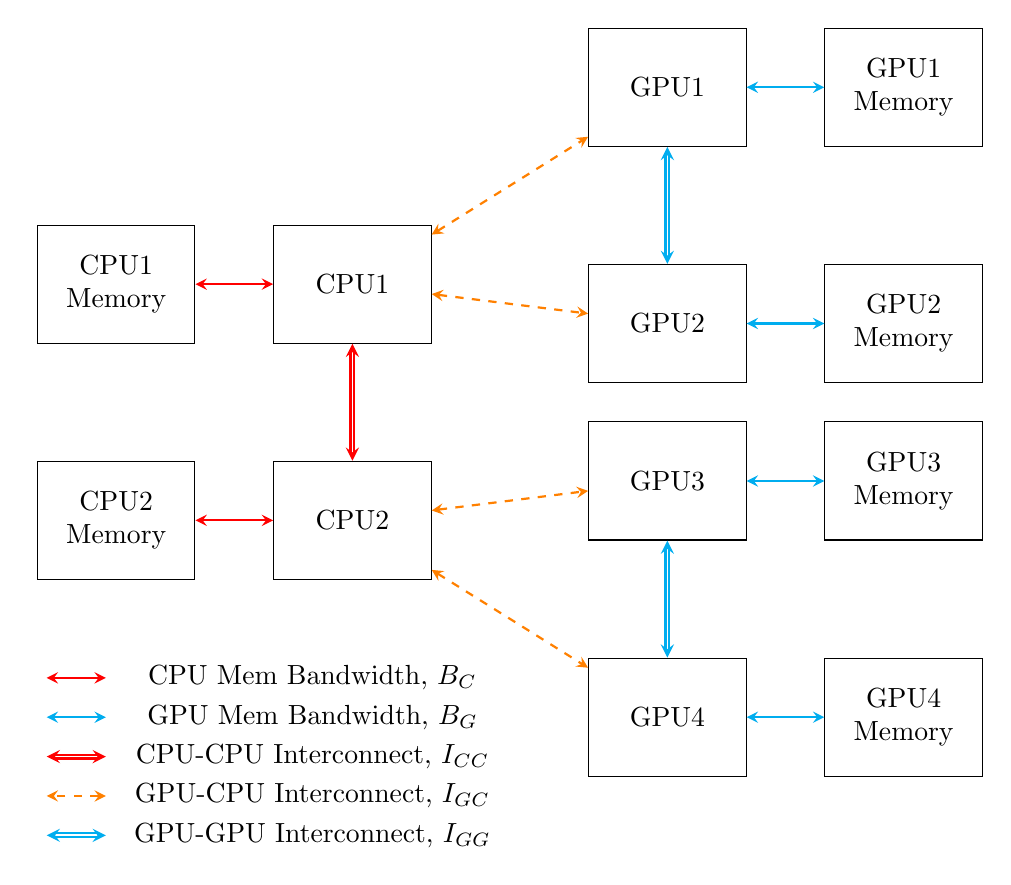
\begin{tikzpicture}
			
			\node[rectangle,
			draw = black,
			text = black,
			anchor = west,
			fill = white,
			align=center,
			minimum width = 2cm, 
			minimum height = 1.5cm] (cpu1) at (0cm,1.5cm) {CPU1};
			
			\node[rectangle,
			draw = black,
			text = black,
			anchor = west,
			fill = white,
			align=center,
			minimum width = 2cm, 
			minimum height = 1.5cm] (cpu2) at (0cm,-1.5cm) {CPU2};
			
			\node[rectangle,
			draw = black,
			text = black,
			anchor = west,
			fill = white,
			align=center,
			minimum width = 2cm, 
			minimum height = 1.5cm] (cpum1) at (-3cm,1.5cm) {CPU1 \\ Memory};
			
			\node[rectangle,
			draw = black,
			text = black,
			anchor = west,
			fill = white,
			align=center,
			minimum width = 2cm, 
			minimum height = 1.5cm] (cpum2) at (-3cm,-1.5cm) {CPU2 \\ Memory};
			
			
			\node[rectangle,
			draw = black,
			text = black,
			anchor = west,
			fill = white,
			align=center,
			minimum width = 2cm, 
			minimum height = 1.5cm] (gpu1) at (4cm,4cm) {GPU1};
			
			\node[rectangle,
			draw = black,
			text = black,
			anchor = west,
			fill = white,
			align=center,
			minimum width = 2cm, 
			minimum height = 1.5cm] (gpu2) at (4cm,1cm) {GPU2};
			
			\node[rectangle,
			draw = black,
			text = black,
			anchor = west,
			fill = white,
			align=center,
			minimum width = 2cm, 
			minimum height = 1.5cm] (gpu3) at (4cm,-1cm) {GPU3};
			
			\node[rectangle,
			draw = black,
			text = black,
			anchor = west,
			fill = white,
			align=center,
			minimum width = 2cm, 
			minimum height = 1.5cm] (gpu4) at (4cm,-4cm) {GPU4};
			
			\node[rectangle,
			draw = black,
			text = black,
			anchor = west,
			fill = white,
			align=center,
			minimum width = 2cm, 
			minimum height = 1.5cm] (gpum1) at (7cm,4cm) {GPU1 \\ Memory};
			
			\node[rectangle,
			draw = black,
			text = black,
			anchor = west,
			fill = white,
			align=center,
			minimum width = 2cm, 
			minimum height = 1.5cm] (gpum2) at (7cm,1cm) {GPU2 \\ Memory};
			
			\node[rectangle,
			draw = black,
			text = black,
			anchor = west,
			fill = white,
			align=center,
			minimum width = 2cm, 
			minimum height = 1.5cm] (gpum3) at (7cm,-1cm) {GPU3 \\ Memory};
			
			\node[rectangle,
			draw = black,
			text = black,
			anchor = west,
			fill = white,
			align=center,
			minimum width = 2cm, 
			minimum height = 1.5cm] (gpum4) at (7cm,-4cm) {GPU4 \\ Memory};
			
			
			\draw[red,  thick, stealth-stealth] (cpum1) to (cpu1);
			\draw[red,  thick, stealth-stealth] (cpum2) to (cpu2);
			\draw[red, double,  thick, stealth-stealth] (cpu1) to (cpu2);
			
			
			\draw[orange, dashed,  thick, stealth-stealth] (cpu1) to (gpu1);
			\draw[orange, dashed,  thick, stealth-stealth] (cpu1) to (gpu2);
			\draw[orange, dashed,  thick, stealth-stealth] (cpu2) to (gpu3);
			\draw[orange, dashed,  thick, stealth-stealth] (cpu2) to (gpu4);
			
			\draw[cyan,  thick, stealth-stealth] (gpum1) to (gpu1);
			\draw[cyan,  thick, stealth-stealth] (gpum2) to (gpu2);
			\draw[cyan,  thick, stealth-stealth] (gpum3) to (gpu3);
			\draw[cyan,  thick, stealth-stealth] (gpum4) to (gpu4);
			
			\draw[cyan, double,  thick, stealth-stealth] (gpu1) to (gpu2);
			\draw[cyan, double,  thick, stealth-stealth] (gpu3) to (gpu4);
			
			
			\node(al) at (-2cm, -3.5cm) {};
			\node (ar) at (-3cm, -3.5cm) {};
			\node[align=left] () at (0.5cm, -3.5cm) {CPU Mem Bandwidth, $B_{C}$};
			\draw[red,  thick, stealth-stealth] (al) to (ar);
			
			\node(al) at (-2cm, -4cm) {};
			\node (ar) at (-3cm, -4cm) {};
			\node[align=left] () at (0.5cm, -4cm) {GPU Mem Bandwidth, $B_{G}$};
			\draw[cyan,  thick, stealth-stealth] (al) to (ar);
			
			\node (bl) at (-2cm, -4.5cm) {};
			\node (br) at (-3cm, -4.5cm) {};
			\node[align=left] () at (0.5cm, -4.5cm) { CPU-CPU Interconnect, $I_{CC}$};
			\draw[red, double,  thick, stealth-stealth] (bl) to (br);
			
			\node (cl) at (-2cm, -5cm) {};
			\node (cr) at (-3cm, -5cm) {};
			\node[align=left] () at (0.5cm, -5cm) { GPU-CPU Interconnect, $I_{GC}$};
			\draw[orange, dashed,  thick, stealth-stealth] (cl) to (cr);
			
			\node (dl) at (-2cm, -5.5cm) {};
			\node (dr) at (-3cm, -5.5cm) {};
			\node[align=left] () at (0.5cm, -5.5cm) { GPU-GPU Interconnect, $I_{GG}$};
			\draw[cyan, double,  thick, stealth-stealth] (dl) to (dr);
			
			
		\end{tikzpicture}
	\end{center}
\caption{Illustration of the universal computing model}
\end{figure}

\subsection{Supercomputers}

For Piz Daint, Summit and Eiger we have collected all relevant hardware metrics and compiled it into the table seen in table \ref{fig:datapoints}. Piz Daint and Eiger were chosen, because we have the possibility to test the Code on its systems. Furthermore we include Summit as its is at the time of writing this thesis, one of the most capable supercomputers in the world.

\small
\begin{table}[H]
	\begin{center}
		\resizebox{\textwidth}{!}{%
		\begin{tabular}{|@{} c | c | c | c | }
			Constant & Piz Daint \cite{piz_daint} & Summit\cite{summit} & Alps (Eiger) \\ 
			\hline
			\# Nodes & 5704 & 4608 & 1024\\
			\# CPUs & 1 & 2 & 2\\
			CPU Model & Intel E5-2690 v3 \cite{E5-2690} & IBM POWER9 & AMD EPYC 7742\cite{AMDEPYC} \\
			CPU Mem. & 64 GB & 256 GB & ?? \\   
			$B_C$  & 68 GB/s & 170 GB/s & 204.8 GB/s x 2	\\
			$I_{CC}$ & - & 64 GB/s & ?? \\
			Base $GHZ_C$ & 2.9 GHZ & 4 GHZ & 2.25 GHZ\\
			Max $GHZ_C$ & 3.8 GHZ & 4 GHZ & 3.4 GHZ\\
			\# Cores & 12 & 22 & 64 \\
			Architexture & Haswell & POWER9 & AMD Infinity Architecture \\
			SIMD & AVX2 & ? & AVX2 \\ 
			\# GPUs & 1 & 6 & 0 \\
			GPU Model & NVIDIA P100 \cite{TESLAP100} &NVIDIA V100s \cite{NVIDIA} & - \\
			GPU Mem. Cap. & 16 GB & 16 GB $\times$ 6 & -\\
			$B_G$ & 732 GB/s & 900 GB/s $\times$ 6 & -\\
			$I_{GC}$ & 32 GB/s & 50 GB/s $\times$ 6 & -\\
			$I_{GG}$ & - & 50 GB/s & -\\
			GPU Tflops & 9,3 & 16.5 & -\\
			\# CUDA Cores & 3584 & 5120 & -\\
		\end{tabular}}	
	\end{center}
	\caption{Datapoints of Supercomputers}
	\label{fig:datapoints}
\end{table}



\subsection{Roofline Performance Model} \label{sec:roof}

In a first step we determine weather our computations are bound by memory bandwidth or the actual performance of the computing unit. The most costly computation is line 6 of the cut method (figure \ref{proc:cut}) with a runtime of $O(32 \times N)$. Oftentimes when an algorithm iterates over a large dataset performing only very little calculations on its individual elements, the limiting factor is the memory. To support this claim make roofline models for all three systems and check weather they are really memory bound. A roofline model compares arithmetic intensity in flops per byte against the actual performance of the computing chip in flops. Therefore we need to gather all the relevant data first.

\subsubsection{Estimating Flops}

For modern hardware, its fairly uncommon to release flops (floating point operations per second) values. Steadily evolving SIMD instruction sets result in varying performance for different implementation details, which in turn are compiled into different assembly instructions. Depending on the algorithm, implementation details and compilation flags the c++ compiler tries to compile ideal assembly instruction sets. SIMD instructions can only be used when there is a contiguous memory access, thus in some cases a poor memory layout choice may lead to a much lower flops. 

For most modern CPU chip architectures AVX is the fastest SIMD instruction set available. The common AVX2 enables the processing of 8 floating point operations per instruction with a  CPI (cycles per instructions) of 0.5. The CPI can also vary depending on chip architecture, but to our knowledge all relevant CPU's from figure \ref{fig:datapoints} indeed support a CPI of 0.5 along with AVX2. A lower CPI results in a higher efficiency, as several instructions can be completed in a single cycle. 

We define in equation \ref{eq:avx}, a function to estimate the number of gigaflops for a given hardware. We define GHZ as the gigahertz which can be reached by the CPU, meanwhile $NF$ is the number of floats which can be processed simultaneously using AVX. $CPI$ is as mentioned the cycles per instructions for the AVX instruction set. Finally we have $np$ which is the number of processors, where we assume a perfect parallelization, meaning 100\% of the code can be parallelized.

\begin{center}
	\begin{equation}
		gflops = GHZ * NF * CPI^{-1} * np
	\end{equation}
\label{eq:avx}
\end{center}

Since we have peak flops benchmarks available for the \textit{NVIDIA} P100 and V100s we do not need to make any estimations on the GPU side.

\subsubsection{Estimating Arithmetic Intensity}

Arithmetic intensity is measured in FLOPS per byte or the number of floating point operations which are computed per byte loaded from memory. The count left part from the cut algorithm (line 6) in figure \ref{proc:cut} can be translated to the following isolated c++ code:

\begin{lstlisting}[language=c++, caption=Counting the particles left of a cut plane, label=Minimal Count Left C++]
	for(auto p= startPtr; p<endPtr; ++p) nLeft += *p < cut;
\end{lstlisting}

Where $p$ is a C-style array which stores the particles position and $nLeft$ stores the number of particles which are smaller than $cut$. We can list the operations per loaded float:

\begin{enumerate}
	\item Compare particle to cut
	\item Add result to $nLeft$
	\item Increment pointer $p$
	\item Compare pointer $p$ with $endPtr$
\end{enumerate}

Which results in a total of 4 operations. Since a single float is stored using 4 bytes, this computes to 1.0 operations per byte or an arithmetic intensity of four. 

Estimating the arithmetic intensity for the GPU is a lot more complicated as it can vary a lot depending on the specific implementation details. But for now we will just assume the same arithmetic intensity as we have had for the CPU.

Note that SIMD instructions do not influence the arithmetic intensity, as the number of floating point operations per byte remains the same. We simply perform a set of operations concurrently. What is however influenced by AVX, is the maximum number of GFLOPS which can be processed by the hardware. If we were to ignore AVX, the algorithm would clearly not be bound by memory, as its performance would lack behind the memory bandwidth. For this reason it is important to consider SIMD instructions.

\subsubsection{The Plots}

Lets us compute the maximally achievable gflops for Piz Daint. To do so, we plug in the corresponding datapoints from figure \ref{fig:datapoints} into the formula \ref{eq:avx} for $np = 1, 2$ and $3$.

\begin{center}
	\begin{equation}
		3.8 * 8 * \frac{1}{0.5} * 2 = 121.6 gflops
	\end{equation}
	\label{eq:daintp1}
\end{center}

\begin{center}
	\begin{equation}
		3.8 * 8 * \frac{1}{0.5} * 4 = 243.2 gflops
	\end{equation}
	\label{eq:daintp2}
\end{center}

\begin{center}
	\begin{equation}
		3.8 * 8 * \frac{1}{0.5} * 8 = 486.4 gflops
	\end{equation}
	\label{eq:daintp3}
\end{center}

The results are depicted as horizontal lines in \ref{fig:roofdaint}. The memory bandwidth is plotted as a line with an equivalent slope. Finally we add a dotted line representing the arithmetic intensity of the Count Left procedure. 
To interpret the roofline mode, one has to follow the dotted line starting from the bottom. Weather it intersect with line representing the maximal performance or the memory bandwidth first, gives an indication weather the program is performance or memory bound. 

\begin{figure}[H]
	\begin{center}
		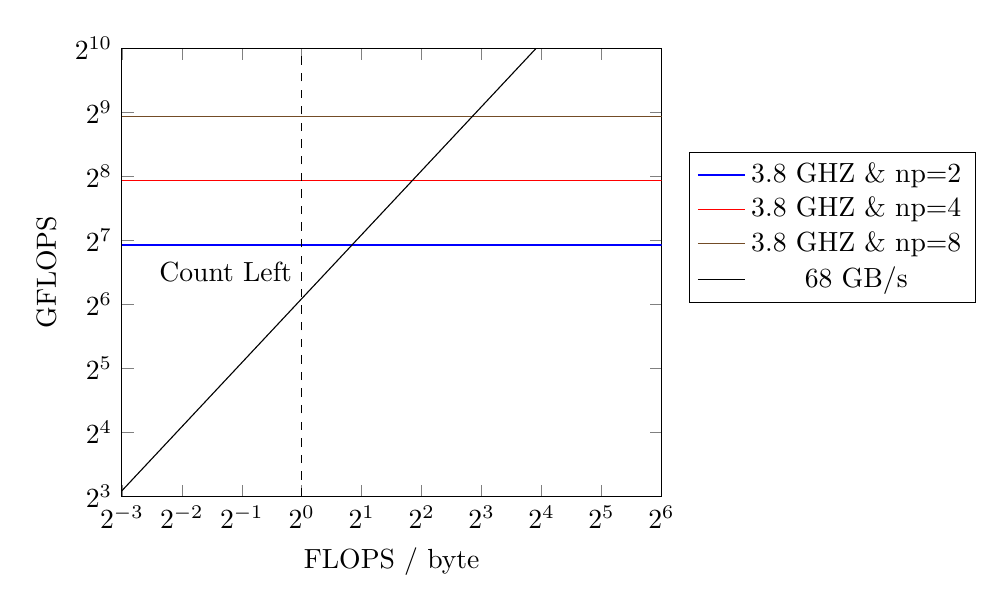
\begin{tikzpicture}
				\begin{axis}[
					xmode=log,
					ymode=log,
					log basis x={2},
					log basis y={2},
					xlabel={FLOPS / byte},
					ylabel={GFLOPS},
					%x filter/.code=\pgfmathparse{#1 + 6.90775527898214},
					xmin = 0.125, xmax = 64, ymin= 8, ymax=1024,
					legend style={at={(1.05,0.6)},anchor=west}]
			
					\addplot+[name path = A, domain = 0.125:64, mark=none] {
						3.8 * 8 * 2 * 2
					};	
					
					\addlegendentryexpanded{3.8 GHZ \& np=2};
					
					\addplot+[name path = A, domain = 0.125:64, mark=none] {
						3.8 * 8 * 2 * 4
					};	
					
					\addlegendentryexpanded{3.8 GHZ \& np=4};
					
					\addplot+[name path = A, domain = 0.125:64, mark=none] {
						3.8 * 8 * 2 * 8
					};	
					
					\addlegendentryexpanded{3.8 GHZ \& np=8};
					
					\addplot+[name path = A, domain = 0.125:64, mark=none] {
						68 * \x
					};	
					
					\addlegendentryexpanded{68 GB/s};
					
		
					\draw[dashed] (axis cs:1,8) -- node[left]{Count Left} (axis cs:1,1024);
					
				\end{axis}
			\end{tikzpicture}
	\caption{Roofline Model for Piz Daint CPU}
	\label{fig:roofdaint}
	\end{center}
\end{figure}


\begin{figure}[H]
	\begin{center}
		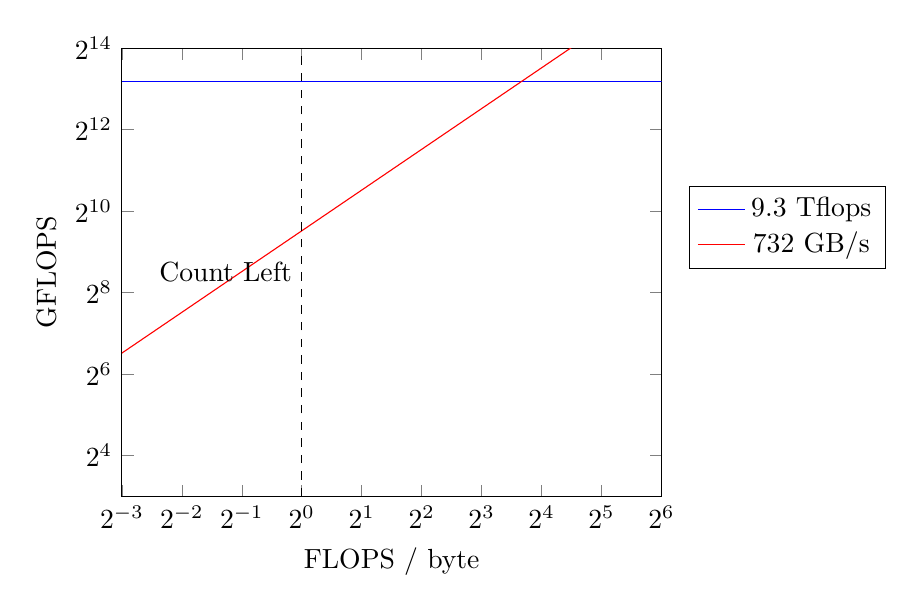
\begin{tikzpicture}
			\begin{axis}[
				xmode=log,
				ymode=log,
				log basis x={2},
				log basis y={2},
				xlabel={FLOPS / byte},
				ylabel={GFLOPS},
				%x filter/.code=\pgfmathparse{#1 + 6.90775527898214},
				xmin = 0.125, xmax = 64, ymin= 8, ymax=16384,
				legend style={at={(1.05,0.6)},anchor=west}]
				
				\addplot+[name path = A, domain = 0.125:64, mark=none] {
					9300
				};	
				
				\addlegendentryexpanded{9.3 Tflops};
				
				\addplot+[name path = A, domain = 0.125:64, mark=none] {
					732 * \x
				};	
				
				\addlegendentryexpanded{732 GB/s};
				
				
				\draw[dashed] (axis cs:1,8) -- node[left]{Count Left} (axis cs:1,16384);
				
			\end{axis}
		\end{tikzpicture}
		\caption{Roofline Model for Piz Daint GPU}
		\label{fig:roofdaintGPU}
	\end{center}
\end{figure}

As it can be seen in figure \ref{fig:roofdaint} and \ref{fig:roofdaintGPU} both the GPU and CPU version running on Piz Daint are memory bound, but due to its much higher memory bandwidth limit, a GPU version should be favored. 

\begin{figure}[H]
	\begin{center}
		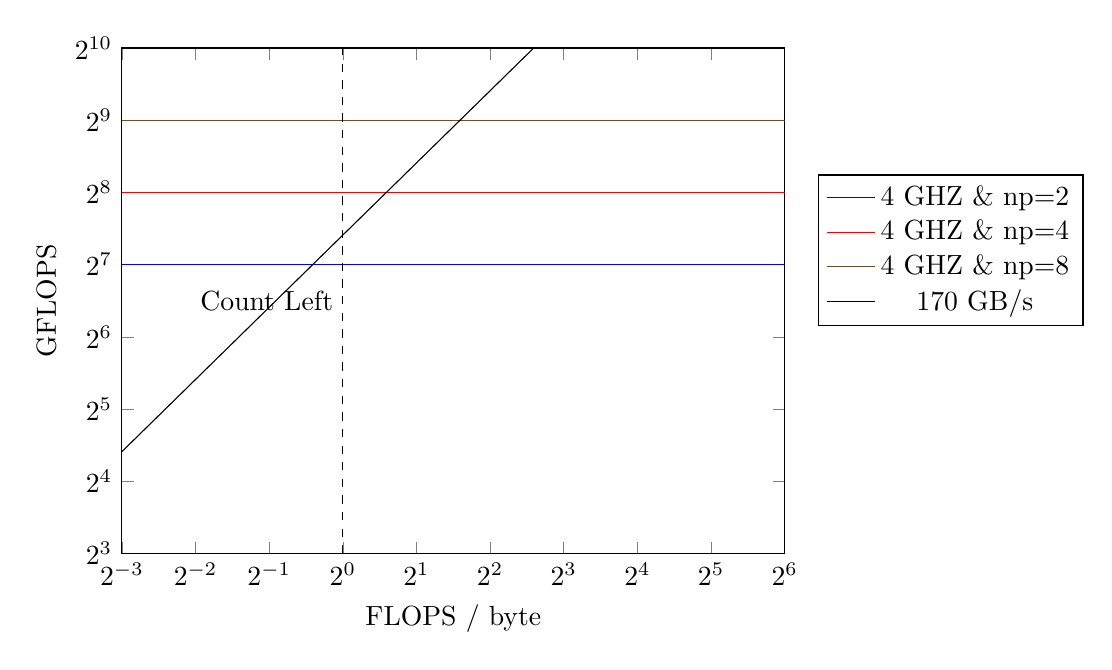
\begin{tikzpicture}
			\begin{axis}[
				xmode=log,
				ymode=log,
				log basis x={2},
				log basis y={2},
				height=8cm,width=10cm, 
				xlabel={FLOPS / byte},
				ylabel={GFLOPS},
				%x filter/.code=\pgfmathparse{#1 + 6.90775527898214},
				xmin = 0.125, xmax = 64, ymin= 8, ymax=1024,
				legend style={at={(1.05,0.6)},anchor=west}]
				
				
				\addplot+[name path = A, domain = 0.125:64, mark=none] {
					4 * 8 * 2 * 2
				};	
				
				\addlegendentryexpanded{4 GHZ \& np=2};
				
				\addplot+[name path = A, domain = 0.125:64, mark=none] {
					4 * 8 * 2 * 4
				};	
				
				
				\addlegendentryexpanded{4 GHZ \& np=4};
				
				\addplot+[name path = A, domain = 0.125:64, mark=none] {
					4 * 8 * 2 * 8
				};	
				
				
				\addlegendentryexpanded{4 GHZ \& np=8};
				
				\addplot+[name path = A, domain = 0.125:64, mark=none] {
					170 * \x
				};	
				
				\addlegendentryexpanded{170 GB/s};
				
				
				\draw[dashed] (axis cs:1,8) -- node[left]{Count Left} (axis cs:1,1024);
			
				
			\end{axis}
		\end{tikzpicture}
	\end{center}
	\caption{Roofline Model for Summit}
	\label{fig:roofsummit}
\end{figure}


\begin{figure}[H]
	\begin{center}
		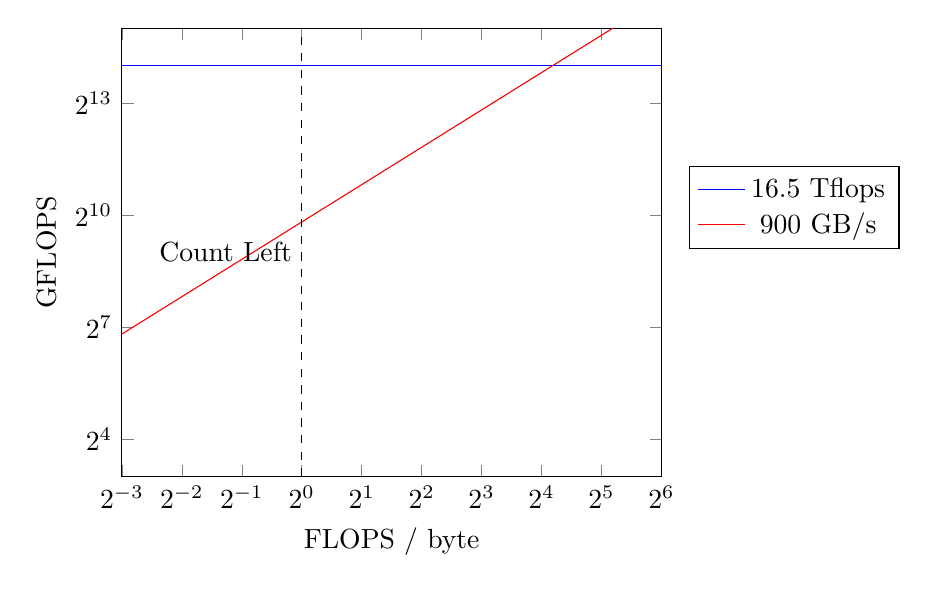
\begin{tikzpicture}
			\begin{axis}[
				xmode=log,
				ymode=log,
				log basis x={2},
				log basis y={2},
				xlabel={FLOPS / byte},
				ylabel={GFLOPS},
				%x filter/.code=\pgfmathparse{#1 + 6.90775527898214},
				xmin = 0.125, xmax = 64, ymin= 8, ymax=32768,
				legend style={at={(1.05,0.6)},anchor=west}]
				
				\addplot+[name path = A, domain = 0.125:64, mark=none] {
					16500
				};	
				
				\addlegendentryexpanded{16.5 Tflops};
				
				\addplot+[name path = A, domain = 0.125:64, mark=none] {
					900 * \x
				};	
				
				\addlegendentryexpanded{900 GB/s};
				
				
				\draw[dashed] (axis cs:1,8) -- node[left]{Count Left} (axis cs:1,32768);
				
			\end{axis}
		\end{tikzpicture}
		\caption{Roofline Model for Summit GPU}
		\label{fig:roofsummitGPU}
	\end{center}
\end{figure}

As visible in figure \ref{fig:roofsummit} and \ref{fig:roofsummitGPU} the same applies to Summit. Its notable how the memory bandwidth only becomes the limiting factor when assuming a parallelization with 4 processors.

\begin{figure}
	[H]
	\begin{center}
		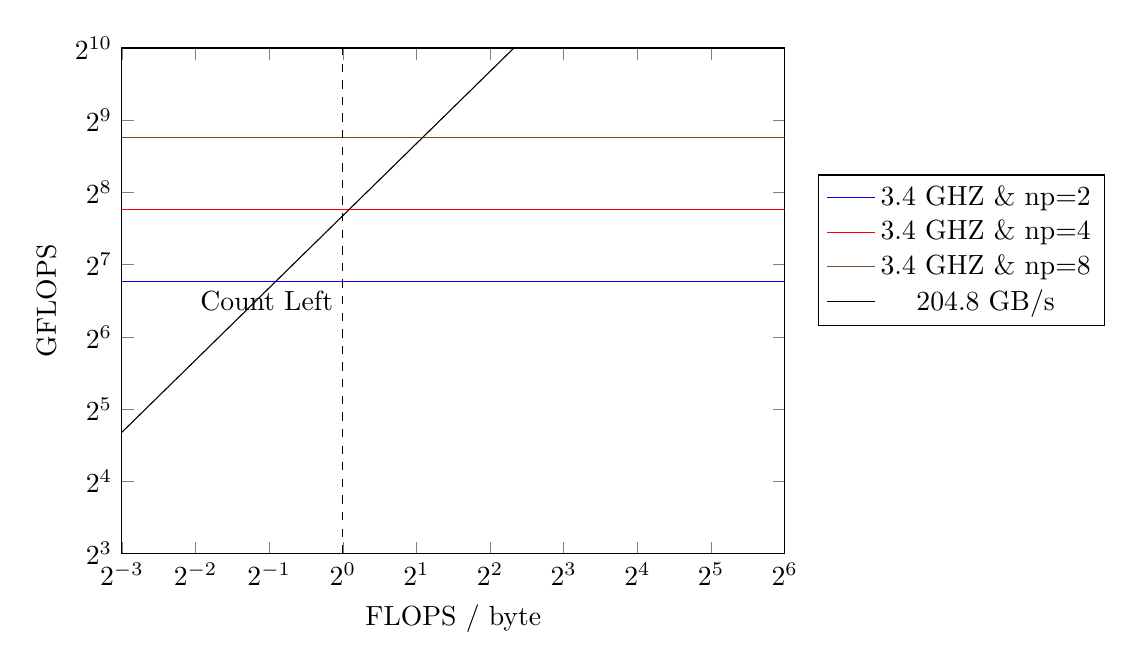
\begin{tikzpicture}
			\begin{axis}[
				xmode=log,
				ymode=log,
				log basis x={2},
				log basis y={2},
				height=8cm,width=10cm, 
				xlabel={FLOPS / byte},
				ylabel={GFLOPS},
				%x filter/.code=\pgfmathparse{#1 + 6.90775527898214},
				xmin = 0.125, xmax = 64, ymin= 8, ymax=1024,
				legend style={at={(1.05,0.6)},anchor=west}]
				
				
				\addplot+[name path = A, domain = 0.125:64, mark=none] {
					3.4 * 8 * 2 * 2
				};	
				
				\addlegendentryexpanded{3.4 GHZ \& np=2};
				
				\addplot+[name path = A, domain = 0.125:64, mark=none] {
					3.4 * 8 * 2 * 4
				};	
				
				\addlegendentryexpanded{3.4 GHZ \& np=4};
				
				\addplot+[name path = A, domain = 0.125:64, mark=none] {
					3.4 * 8 * 2 * 8
				};	
				
				\addlegendentryexpanded{3.4 GHZ \& np=8};
				
				\addplot+[name path = A, domain = 0.125:64, mark=none] {
					204.8 * \x
				};	
				
				\addlegendentryexpanded{204.8 GB/s};
				
				\draw[dashed] (axis cs:1,8) -- node[left]{Count Left} (axis cs:1,1024);
				
				
			\end{axis}
		\end{tikzpicture}
	\end{center}
	\caption{Roofline Model for Alps}
	\label{fig:roofalps}
\end{figure}

Finally alps, which has the highest memory bandwidth compared to its flops, also becomes limited by the bandwidth after using more than four processors.

\subsubsection{Empirical Verification}

We consider a minimal C++ code to verify the theoretical model. We use the -S flag along with the g++ compiler to generate assembly code from the c++ source code and make sure that AVX commands are enabled. For testing purposes all entries in the array are set to random values between 0 and 1, and cut is set to 0.5.

In a first test, we do not enable AVX, but turn on $O3$. The generated assembly code is depicted in listing \ref{assembler}.

\begin{lstlisting}[language=c++, caption=Reduction Assembler Code without AVX, label=assembler]
.L18:
	movups	(%rax), %xmm0
	addq	$16, %rax
	cmpltps	%xmm2, %xmm0
	psubd	%xmm0, %xmm1
	cmpq	%rdx, %rax
	jne	.L18

\end{lstlisting}

$psubd$ is a packaged instruction, meaning it already uses some form of SIMD instructions. The command is used in the MME and later the SSE2 instruction set. Since we can observe that the $xmm$ registers are used, we know its a SSE2 instruction. 

If we additionally set the compile flag -march=native we end up with the instructions as depicted in listing \ref{assembler-avx}.

\begin{lstlisting}[language=c++, caption=Reduction Assembler Code with AVX2, label=assembler-avx]
.L19:
	vmovups	(%rax), %ymm3
	addq	$32, %rax
	vcmpltps	%ymm2, %ymm3, %ymm0
	vpsubd	%ymm0, %ymm1, %ymm1
	cmpq	%rdx, %rax
	jne	.L19	

\end{lstlisting}

We can identify $vmovups$, $vcomplpts$ and $vpsubd$ which are AVX commands. Since they are using the ymm instead of the xmm registers, we know these are AVX2 and not AVX commands.

The following results were obtained on $2^{27}$ particles with a thread count of 16 on Piz Daint. The reduction takes 2.3 milliseconds, resulting in a throughput of $2^{27} / 10^{9} * 10^3 / 2.3 = 58 gflops$. This is close to the memory bandwidth (68 GB/s) and far below the performance maximum of the CPU, which even for ($np = 1$) is $3.8 * 8 * 2 * 1 * 16 = 972.8 gflops$. Thus we conclude that the algorithm is memory bound for the CPU and most probably memory bound for the GPU. 


\subsection{Runtime Estimates}

We construct runtime estimation for the CPU version and two different GPU implementations. In the first GPU implementation \textit{GPU Counting}, we simply send an array of particles to the GPU, where counting is then performed. In a more advanced variant \textit{GPU Counting and Partitioning} we send the particles from the CPU to GPU only once and perform the partitioning on the GPU as well.  

We assume a precision $p$ of 32, which is general standard for both integers and floats and its a sensible assumption for astrophysical simulations. The total storage required for all particle positions is $32 \times 3 \times N bits = 4 \times 3 \times N Bytes = 12 \times N Bytes$. Furthermore we assume $d = 1024$ and $N=10^9$.
 
\subsubsection{CPU Version}


Whilst the number of cells increases each time the tree depth is increased, simultaneously the number of particles to be iterated over decreases. Thus the amount of cells which are to be iterated cancels out and we end up with the size of all particles $s$ divide by the memory bandwidth $B_C$.  


Each time the leaf cells of the SPTDS are split into two child cells and appended to the tree, we end up with twice the number of leaf cells. Considering we want to end up with $d$ leaf cells in the end, we need to perform the cut algorithm $\lceil log_2(d) \rceil$ times for all leaf cells. 

Consequently we sum over all $\lceil log_2(d) \rceil$ iterations, where in each iteration a cut has to be found for $i$ cells. The cut itself is found in $p$ iterations, where the actual array of particles is each time we grow the SPTDS by a level. As only the memory bandwidth is considered, we divide the size of the particles to be iterated over.

\begin{center}
	\begin{equation}
		\sum_{i=1}^{\lceil \log_2{d} \rceil} i \times p \times  \frac{ \frac{s}{i}}{B_C} 
		\label{eq:cpu1}
	\end{equation}
\end{center}

$i$ cancels out from the equation and we end up with:

\begin{center}
	\begin{equation}
		\sum_{i=1}^{\lceil \log_2{d} \rceil} p \times \frac{s}{B_C} 
		\label{eq:cpu2}
	\end{equation}
\end{center}

Which can be simplified to:

\begin{center}
	\begin{equation}
		\lceil \log_2(d) \rceil  \times \left ( p \times \frac{ s }{B_{C}} \right )
		\label{eq:cpu}
	\end{equation}
\end{center}

\subsubsection{GPU Counting}


The Equation \ref{eq:gpu} for the GPU is similar, the only difference being that we use the GPU memory bandwidth $B_{GPU}$ instead of the CPU bandwidth. Furthermore we have to consider the time it takes to send the data from the CPU to the GPU. This adds the terms size divided by CPU to GPU memory bandwidth denoted as $I_{GC}$.

\begin{center}
	\begin{equation}
			\lceil log(d) \rceil \times \left ( p \times \frac{s}{B_{G}} +\frac{s}{I_{GC}} \right ) 
		\label{eq:gpu}
	\end{equation}
\end{center}


\subsubsection{GPU Counting and Partitioning}\label{gpu-tree-building}

We can also consider performing the partitioning on the GPU, this means that there is no need to send data from the CPU to GPU each time we want to find a cut, allowing us to reduce the costly overheads. This means that we are able to move the corresponding terms out of the brackets. 

\begin{center}
	\begin{equation}
		\lceil log(d) \rceil \times \left ( p \times \frac{s}{B_{G}} \right ) + \frac{s}{I_{GC}} = t
		\label{eq:gputree}
	\end{equation}
\end{center}

\newcommand\s{12}

\newcommand\p{32}

%\newcommand\d{1024}

\normalfont
\subsubsection{Plugin Values} 

Let us plugin the values from figure \ref{fig:datapoints} into the corresponding formulas \ref{eq:cpu}, \ref{eq:gpu} and \ref{eq:gputree} for Piz Daint.
The naive implementation yields the following speeds for the naive CPU  implementation:

\pgfmathsetmacro\cpuPiz{ln(1024) / ln(2) * (\p * \s / 68)}

\begin{center}
	\begin{equation}
		\lceil log(1024) \rceil \times \left ( \p \times \frac{ \s GB }{68 GB/s} \right )  = \cpuPiz s
	\end{equation}
\end{center}


And the corresponding GPU implementation:
\pgfmathsetmacro\gpuPizN{ ln(1024) / ln(2) * (\p * \s / 732 + \s / 32)}
\begin{center}
	\begin{equation}
		\lceil log(1024) \rceil \times \left ( 32 \times \frac{12 GB}{732 GB/s} + \frac{12 GB}{32 GB/s} \right )=  \gpuPizN s
	\end{equation}
\end{center}

This yields in a speed-up of:
\pgfmathsetmacro\speedup{\cpuPiz / \gpuPizN}
\begin{center}
	\begin{equation}
		\frac{\cpuPiz}{\gpuPizN} = \speedup \times
	\end{equation}
\end{center}


When considering the GPU Counting and Partitioning we end up with:
\pgfmathsetmacro\gpuPizT{ ln(1024)/ln(2) * (\p * \s / 732)  + \s / 32}
And the corresponding GPU implementation:
\begin{center}
	\begin{equation}
		\lceil log(1024) \rceil \times \left ( \p \times \frac{\s GB}{732 GB/s} \right ) + \times \frac{\s GB}{32 GB/s} = \gpuPizT s
	\end{equation}
\end{center}

This yields in a speed-up of:
\pgfmathsetmacro\speedup{\cpuPiz / \gpuPizT}
\begin{center}
	\begin{equation}
		\frac{\cpuPiz}{\gpuPizT} = \speedup \times
	\end{equation}
\end{center}

\vspace{5mm}

\pgfmathsetmacro\cpuSummit{ln(1024) / ln(2) * (\p * \s / (170 * 2)}
\pgfmathsetmacro\gpuSummitN{ln(1024) / ln(2) * (
	(\p * \s / (900 * 6) + 
	\s / (50 * 6)
	)}
\pgfmathsetmacro\gpuSummitT{ln(1024) / ln(2) * 
	(\p * \s / (900 * 6))
	+  \s / (50 * 6)}
\pgfmathsetmacro\cpuEiger{ln(1024) / ln(2) * (\p * \s / (204.8 * 2)}


\begin{comment}

\subsection{Summit}

Let us plugin the values from Figure \ref{fig:datapoints} into the corresponding formulas \ref{eq:cpu}, \ref{eq:gpu}, \ref{eq:cputree} and \ref{eq:gputree}.

\subsubsection{Naive implementation}
The naive implementation yields the following speeds for the naive CPU  implementation:


\begin{center}
	\begin{equation}
		log(1024) \times \left ( \p \times \frac{ \s GB }{170 GB/s \times 2} \right ) = \cpuSummit s
	\end{equation}
\end{center}

And the corresponding GPU implementation:

\begin{center}
	\begin{equation}
		log(1024) \times \left ( \p \times \frac{\s GB}{900 GB/s \times 6} + \frac{\s GB}{50 GB/s \times 6}  + \frac{\s GB}{170 GB/s \ \times 2} \right )= \gpuSummitN s
	\end{equation}
\end{center}

This yields in a speed-up of:
\pgfmathsetmacro\speedup{\cpuSummit / \gpuSummitN}
\begin{center}
	\begin{equation}
		\frac{\cpuSummit s}{\gpuSummitN s} = \speedup \times 
	\end{equation}
\end{center}


\subsubsection{GPU Tree Building}

And the corresponding GPU implementation:

\begin{center}
	\begin{equation}
		log(1024) \times \left ( \p \times \frac{\s GB}{900 GB/s \times 6} \right ) + \frac{\s GB}{50 GB/s \times 2}  + \frac{\s GB}{170 GB/s \times 2} = \gpuSummitT s
	\end{equation}
\end{center}

This yields in a speed-up of:
\pgfmathsetmacro\speedup{\cpuSummit / \gpuSummitT}
\begin{center}
	\begin{equation}
		\frac{\cpuSummit s}{\gpuSummitT s} = \speedup \times
	\end{equation}
\end{center}


\vspace{5mm}


\subsection{Eiger}

\pgfmathsetmacro\cpuEiger{ln(1024) / ln(2) * (\p * \s / (204.8 * 2)}

\begin{center}
	\begin{equation}
		\log(1024) \times \p \times \frac{ \s GB }{204.8 GB/s \times 2} = \cpuEiger s
	\end{equation}
\end{center}

\end{comment}

\subsection{Conclusion}

 
The computations for Eiger and Summit can analogously to the ones from Piz Daint. For Eiger we cannot make any assumption for a GPU version as its CPU only system. All the results are plotted in \ref{fig:exectimes}. As expected the GPU Counting outperforms the CPU version on both hybrid (CPU and GPU available )super computers. Furthermore GPU Counting and Partitioning yields more performance improvements, but the speed up is less drastic. As the model may differ from reality depending in implementation and compilation details, these results cannot be taken for granted and we will compare the results with actual empirical observations in section \ref{sec:empan}. 

\begin{figure}[H]
	\begin{center}
		\begin{tikzpicture}
			
			\begin{axis} [ybar,height=10cm,width=13cm, 
				bar width=0.8cm,
				enlargelimits=0.2,
				symbolic x coords={Piz, Summit, Eiger},
				legend columns=1,
				legend entries={CPU, Hybrid Naive, Hybrid Tree},
				ylabel={Runtime (s) },
				x tick label style={rotate=45,anchor=east}, 
				xtick=data]
				\addplot coordinates {
					(Piz,\cpuPiz ) 
					(Summit,\cpuSummit) 
					(Eiger,\cpuEiger) 
				};
			
				\addplot coordinates {
					(Piz,\gpuPizN ) 
					(Summit,\gpuSummitN ) 
				};
			
				\addplot coordinates {
					(Piz,\gpuPizT ) 
					(Summit,\gpuSummitT  ) 
				};
			\end{axis}
			
		\end{tikzpicture}
	\end{center}

\caption{Execution times of different strategies}
\label{fig:exectimes}
\end{figure}


\newpage
\section{CPU Implementation}

In this section we describe the stand-alone implementation of the ORB algorithm using CPU acceleration only. Building on the CPU version, we later introduce GPU accelerated alternatives to selected parts of the code. 

We develop somewhat separately from the PKDGrav codebase in order to keep the project smaller and more easy to understand. However we make use of the machine dependent layer (MDL) from PKDGrav, which is used to distribute the workload among processors. This reduces the complexity of the implementation and we do not have to worry about communication methods and CPU parallelism too much. Furthermore it makes integration into PKDGrav simple. Note that processors might be located in different nodes, but MDL is general enough to abstract node and processor level communication and parallelization away.

We refrain from describing each part of the code in detail, however any details crucial to performance are described. Furthermore, we will pay special attention to the CUDA kernels and also memory management strategies for several reasons: minor implementation details can have a big impact upon the performance and increased replicability.

For this project we will use C++ 17 along with CUDA 11.3, OpenMPI 4.1.0 and Blitz++ 1.0.2 \cite{blitzcpp}. 

\subsection{MDL and PKDGrav}

MDL, the machine dependent layer provides an abstraction layer around the parallel primitives introduced by PKDGrav. The Master layer is responsible to coordinate the flow of the program. It does so by calling the PST (Processor Set Tree), which distributes the tasks and gets processors to work on them. As the name suggests, the PST is organized as a binary tree where intermediate nodes contains a pointer to a consecutive processor as well as a next lower node. Each leaf cell of the graph then correspond to an individual processor.

Parallel processes are dispatched by descending the PST until they reach all processors. There computations are performed and the results are combined by passing them back up the PST until they reach the master.
A parallel process can be programmed by implementing the service interface as explained in section \ref{services}.

Each processor has its own local data, which can be accessed by calling $pst->lcl$. 

\subsection{Particles}

The particles array has ownership over all particle objects. It has a (N,3) shape where each row represents a single particle. To enable coalesced memory access when iterating over a single axis i.e. $x_{:, axis}$, we choose a column major storage order, over a row major storage order. Even though row accesses patterns i.e. $x_{i,:}$ are used as well, they happen less frequently. Most importantly there are cases where entire section of a row have to copied, which is by magnitude faster with row major storage.

We use C-style arrays interchangeably with Blitz++ arrays to store all particles. Blitz++ is an open source wrapper class around C-style arrays, which helps with pointer management and can speed up the debugging process by keeping track of the array boundaries. Furthermore it features array slicing and does its own memory management. In certain cases we need to access the actual C-style array, which can be accessed with $array.data()$. For example when iterating over the Blitz++ array, we have observed compiled assembly code  which does not reflect the latest SIMD instructions.

The particle data is loaded into the local data storage of each processor, meaning each processor owns a different unique set of particles.

\subsection{Cell}

The cell class is a structure keeping track of the fundamental cell information. In essence it is the analogue to the concept of the $cell$ which we have already introduced in section \ref{section:orb}.

Quickly building and accessing elements of the SPTDS generated by ORB requires a suitable data structure. Instead of a tree with pointers, we can use a heap since the necessary conditions for a nearly complete binary tree are met. Elements within a heap can be accessed and added in constant runtime. Depicted in figure \ref{fig:treeheap} is the finished SPTDS of the sample dataset stored as a heap.

The SPTDS and thus the cells are constructed on the master alone, cells are only distributed when dispatching services on the PST.

\begin{figure}[H]
	\begin{center}
		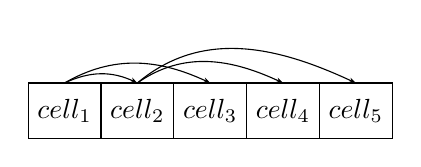
\begin{tikzpicture}[
			%  -{Stealth[length = 2.5pt]},
			start chain = going right,
			node distance = 0pt,
			MyStyle/.style={draw, minimum width=2em, minimum height=2em, 
				outer sep=0pt, on chain},
			]
			\node [MyStyle] (1) {$cell_1$};
			\node [MyStyle] (2) {$cell_2$};
			\node [MyStyle] (3) {$cell_3$};
			\node [MyStyle] (4) {$cell_4$};
			\node [MyStyle] (5) {$cell_5$};
			\begin{scope}[-{Stealth[length = 2.5pt]}]
				\draw (1.north) [out=25, in=155] to (2.north);
				\draw (1.north) [out=30, in=155] to (3.north);
				\draw (2.north) [out=35, in=155] to (4.north);
				\draw (2.north) [out=40, in=155] to (5.north);
			\end{scope}
		\end{tikzpicture}
		\qquad
		\begin{figure}
			\Tree[.cell_1 [.cell_2 [.cell_4 ] [.cell_5 ] ]
			[.cell_3 ]]
		\end{figure}
	\end{center}
	\caption{Tree as heap}
	\label{fig:treeheap}
\end{figure}

An array can be used as an efficient storage medium for the heap, since in our case $d$ can be set at compile time and the maximum number of cells in the SPTDS can be derived from that. Meaning the array can be allocated statically.
Because MDL communicates data as arrays between the threads, another advantage of the array storage is the absence of any costly data structure conversion. 

Since the STPDS is only a nearly complete binary tree and not a complete binary tree, we have to be careful when iterating over the levels of three, as the very last level is not filled entirely with cells. But because $d$ is known, many attributes of the SPTDS can be determined deterministically.

\subsubsection{Heap Conditions}
As with all heap data-structures we have the following conditions:

\begin{itemize}
	\item The root cell has index 1
	\item The left child of cell at index $i$ can be accessed at the index $i\times2$. 
	\item The left child of cell at index $i$ can be accessed at the index $i\times2 + 1$. 
\end{itemize}

\begin{figure}[H]
	\centering
	\begin{forest}
		[$cell_1$
		[$cell_2$ [$cell_4$] [$cell_5$]][$cell_3$]  
		]
	\end{forest}
	\caption{Tree with $d$ = 3}
	\label{fig:extree}
\end{figure}

\vspace{0.5cm}
We can derive the following constraints given the number of leaf cells $d$. 

\begin{itemize}
	\item We can compute the depth of the tree with: $\lceil log_2(d) \rceil$
	\item The number of leaf cells on the second last level is given by $2^{depth} - d$ 
	\item There are exactly $2 \times d - 2^{depth}$ items (which must all be leaf cells) on the last level. 
	\item The total number of cells are $2\times d - 1$.
\end{itemize}

In the example tree depicted in figure \ref{fig:extree} we indeed observe that the depth corresponds to: $\lceil log_2(d) \rceil = 2$, the number of leaves on the second last level is  $2^{2} - 3 = 1$ and the number of leaves on the last level are $2 \times 3 - 2^{2} = 2$. Finally the total number of cells is $2\times 3 - 1 = 5$.

\subsubsection{Class}
Among the fields in the cell are the following variables:

\begin{itemize}
	\item $id$: Unique identification of the cell instance. Corresponds to its index in the heap array plus one. The plus one comes from the different indexing for heap constraints, where we start with 1, and the classic array indexing starting with 0. It can be used to compute  indices of both child cells and parent cells using the above shown formulas.
	\item $nLeafCells$: Equivalent to  $d_{cell}$ and depicts the number of leaf cells to be found in all of its successors. Its used when building the tree, to track weather a cell needs to be split or not. 
	\item $lower$: 3D point coordinate representing the lower boundary corner of the 3D volume $V_{cell}$ which is encompassed by this cells.
	\item $upper$: Represents the upper boundary corner of the volume.	
	\item $cutAxis$: Axis where the cell is to be cut. 
\end{itemize}

To support and simplify common operations, a further abstraction layer is given with the following functions:


\begin{itemize}
	\item $setCutAxis()$: Evaluates the proper $cutAxis$ given the $upper$ and $lower$ variables.
	\item $cut()$: Cuts the cell and returns two new cells. 
	\item $lower$: 3D point coordinate representing the lower boundary corner of the 3D volume $V_{cell}$ which is encompassed by this cells.
	\item $getLeftChildId()$: Returns the ID of the left child cell, meaning its volume is in the cut axis smaller than the cut plane. 
	\item $getRightChildId()$: The equivalent for the right child. 
\end{itemize} 

\subsection{Mapping Cells to Particles}

As SPTDS heap is stored on the master but the particles are distributed among the local storages of the processors, its is crucial to know which particles are encompassed in the volume of which cell. Thus we introduce a data structure to keep track of the relation between cells and its particles. 
Thanks to the partitioning algorithm all particles belonging to a single cell can be found in a consecutive section of the particles array. Thus we can use a 2D array, which again is stored in the local data of the processor, where for each cell the corresponding range is stored as a tuple. Making the size of the array equivalent to the total number of cells $2 \times d -1$ multiplied by two. Naturally the data structure needs to be updated across all processors whenever we a partition is performed.

\subsection{Services}\label{services}

A service implementation consists of a $Service()$ function as well as a $Combine()$ function. Parameters include an $PST$ object which stores information about the process location as well as the local data. Furthermore two void pointers providing storage for the input and output data called $in$ and $out$ along with their respective sizes are passed. The reason void pointers are used, is the variability of the input data structure but c++ does not offer dynamic typing. Data stored inside the void pointers can be converted into their respective classes using casting. 

In the $Combine()$ function two output void pointers $vout$ and $vout2$ and the sizes of the underlying arrays are given as parameters. A combination strategy of the elements can be chosen and implemented, where the results is to be stored in $vout$. For example if we were to implement a service which returns the sum of all particles, the combine function would simply store the sum of $vout$ and $vout2$ in $vout$.

\subsubsection{Init and Finalize Service}

All data stored as local data, which is not managed by Blitz++, must be allocated when initializing and after the program has finished, the memory is freed to avoid any leaks. Allocation and freeing is not free of cost, thus it makes sense to reuse memory whenever possible. 

The initialize service is also responsible to load the particle data into the local memory of each PST. 

\subsubsection{Count Left Service}

As mentioned, counting the elements smaller than the cut position is computationally intensive. T
The $Service()$ function which performs the actual computations, $in$ points to an array of cells and as we know the length of the array, we can simply iterate over all of its elements and cast them to the correct cell data structure as shown in listing \ref{ctl} on line 1-2. In case the $foundCut$ flag of cell was set to true, we know that the ideal cut was already found and we can continue with the next cell (line 4-6).
We then read the begin and end indices of the particles array corresponding to the range of objects contained within the cells volume and respectively make a slice of the local particles array (lines 7-11). We then compute start and end pointers and obtain the cut position to be tested (lines 13 -17). Finally the number of particles smaller than the cut are counted and written back to the output array (lines 18-23). As we need to store the results for each cell individually, the output is stored at an offset equivalent to the $cellPtrOffset$. This offset however does not corresponds to the $cell.id$, its rather a sequential indexing over all leaf cells of the same depth in the SPTDS. 


\begin{lstlisting}[language=c++, caption=Part of the Count Left Service() method, label=ctl]
for (int cellPtrOffset=0; cellPtrOffset<nCells; ++cellPtrOffset){
	auto cell = static_cast<Cell>(*(in + cellPtrOffset));
	
	if (cell.foundCut) {
		continue;
	}
	int beginInd = pst->lcl->cellToRangeMap(cell.id, 0);
	int endInd =  pst->lcl->cellToRangeMap(cell.id, 1);
	
	blitz::Array<float,1> particles =
	pst->lcl->particlesAxis(blitz::Range(beginInd, endInd));
	
	float * startPtr = particles.data();
	float * endPtr = startPtr + (endInd - beginInd);
	
	int nLeft = 0;
	float cut = cell.getCut();
	for(auto p= startPtr; p<endPtr; ++p)
	{
		nLeft += *p < cut;
	}
	
	out[cellPtrOffset] = nLeft;
}
\end{lstlisting}

Combining the data is straight forward, as in $Combine()$ $vout$ and $vout2$ contain the counts for a given number of particles. The master requires a global count across all the particles contained within all local storages, therefore each element of $vout$ is summed together with $vout2$. 

\begin{lstlisting}[language=c++, caption=Part of the Count Left Combine() method, label=ctlc]
	for(auto i=0; i<nCounts; ++i)
		out[i] += out2[i];
\end{lstlisting}

\subsubsection{Count}

Counting the total number of particles contained within a cell is trivial with the $cellToRangeMap$. The results can be obtained by subtracting the begin index from the end index of each cell. The $Combine()$ is equal to the one shown for the Count Left Service.

\begin{lstlisting}[language=c++, caption=Part of Count Service() method]
	for (int cellPtrOffset=0; cellPtrOffset<nCells; ++cellPtrOffset) {
		auto cell = static_cast<Cell>(*(in + cellPtrOffset));
		out[cellPtrOffset] = 
		lcl->cellToRangeMap(cell.id,1) - 
		lcl->cellToRangeMap(cell.id,0);
	}
\end{lstlisting}

\subsubsection{Partition}

The Partitioning Service is a direct implementation of the hoare partition and can be seen in listing \ref{partition}. Again the service receives a buffer with a given number of cells, which are then iterated over using the outer for loop. Each cell from the buffer is then casted to the proper struct (line 2). Using the id of the cell, we can the access the start and end indices of the corresponding particles stored in local storage (lines 4-5). Lines 7-37 search for pairs located on the wrong side of the cut and then swap them using a simple $swap()$ helper function. $i$ has to be initialized using $beginInd -1$ as the $i++$ operation happens before a read on the array (line 15). For the same reason $j$ is initialized to $endInd$ and not $endInd -1$. Then the while loop terminates, $i$ points to the first index in the array where the value is greater than the cut, therefore we can update the $cellToRangeMap$ with $i$, as for the left child cell the start remains equal but the end is now $i$ and for the right child cell its vice versa. 
Note that the implementation is not ideal for two reasons:

\begin{enumerate}
	\item The blitz wrapper class should be avoided and instead the memory directly accessed.
	\item In this particular case the column major storage order is not ideal, as rows are accessed over and over again.
\end{enumerate}

\begin{figure}[H] 
	\begin{lstlisting}[language=c++, caption=Partition Service, label=partition]
for (int cellPtrOffset=0; cellPtrOffset<nCells; ++cellPtrOffset){
	auto cell = static_cast<Cell>(*(in + cellPtrOffset));
	
	int beginInd = pst->lcl->cellToRangeMap(cell.id, 0);
	int endInd = pst->lcl->cellToRangeMap(cell.id, 1);
	
	int i = beginInd-1, j = endInd;
	float cut = cell.getCut();
	
	while(true)
	{
		do
		{
			i++;
		} while(lcl->particles(i,cell.cutAxis)<cut and i<=endInd);
		
		do
		{
			j--;
		} while(lcl->particles(j,cell.cutAxis)>cut and j>=beginInd);
		
		if(i >= j) {
			break;
		}
		
		swap(lcl->particles, i, j);
	}
	
	swap(lcl->particles, i, endInd -1);
	
	lcl->cellToRangeMap(cell.getLeftChildId(), 0) =
	lcl->cellToRangeMap(cell.id, 0);
	lcl->cellToRangeMap(cell.getLeftChildId(), 1) = i;
	
	lcl->cellToRangeMap(cell.getRightChildId(), 0) = i;
	lcl->cellToRangeMap(cell.getRightChildId(), 1) =
	lcl->cellToRangeMap(cell.id, 1);
	
}
	\end{lstlisting}
\end{figure}


\subsubsection{Make Axis}

As mentioned in section \ref{sec:multipole} the relevant axis to search for the cut position differs for each cell. Therefore we cannot simply iterate over a single array, we need to iterate over the relevant axis instead. In order to simplify the process we introduce a service which copies iterates over all cells and copies the slice of coordinates which are encompassed in its volume and lie on its cut axis to a temporary array.

\subsection{Parallel Schedule}\label{sec:parellize-orb}

In the context of parallelization, we define the number of processors as $np$ and $p_0$ is the processor executing the master layer. 
Initially we assume that each processor has a random unique subset of all the particles stored in its local memory.

In the running example this might look as follows:

\begin{figure}[H]
	
	\centering
	\begin{tikzpicture}
		\begin{axis}
			[
			nodes near coords,
			xmin=-0.,
			xmax=1.,
			ymin=-0.,
			ymax=1.,
			title=Recursion depth 0,
			legend cell align=left
			]
			
			\addplot    +[
			only marks,
			point meta=explicit symbolic,
			restrict expr to domain={\thisrow{o1}}{0:0}, 
			] table [
			x=x, 
			y=y, 
			meta=id, 
			col sep=comma] 
			{particles10.csv};
			
			\addplot    +[
			only marks,
			point meta=explicit symbolic,
			restrict expr to domain={\thisrow{o1}}{1:1}, 
			] table [
			x=x, 
			y=y, 
			meta=id, 
			col sep=comma] 
			{particles10.csv};
			
			\addplot    +[
			only marks,
			point meta=explicit symbolic,
			restrict expr to domain={\thisrow{o1}}{2:2}, 
			] table [
			x=x, 
			y=y, 
			meta=id, 
			col sep=comma] 
			{particles10.csv};
			
			\legend{$p0$,$p1$,$p3$}
			
			%\draw [fill=red!20](0.0,0.0) rectangle (1, 1);
			%\node[below] at (0.5, 1){$cell_1$};
		\end{axis}
	\end{tikzpicture}
	\caption{Example particles distributed randomly across 3 nodes}
\end{figure}

The Master schedules all other processors but also performs tasks by itself. The exact schedule is illustrated in figure \ref{fig:orbp} where a service which is dispatched from the master and executed on all processors is depicted as a horizontal rectangle. Computations which are only performed by a single processor are represented by a vertical rectangle. 

\begin{figure}[H]
	\begin{center}
		\begin{tikzpicture}
			
			\timeline{6}{13}{3}
			
			
			\parallelloop{-2}{11.5}{8}{1.5}{loop till tree built};
			
			\parallelloop{-1}{9.5}{7}{5.5}{loop till cut found};
			
			\communication{Init}{0}{7}{12};
			
			\communication{Count}{0}{7}{11};
			
			
			\communication{Make Axis}{0}{7}{10};
			
			\communication{Count Left}{0}{7}{9};
			
			\process{improve \\ cut}{0}{8};
		
			
			\communication{Partition}{0}{7}{5};
			
			\communication{Finalize}{0}{7}{1};
			
			\process{generate\\ new \\ cells}{0}{4};
			
		\end{tikzpicture}
	\end{center}
	\caption{Parallelized ORB CPU version}
	\label{fig:orbp}
\end{figure}

\newpage
\section{GPU Implementation}\label{sec:gpuimpl}

CUDA is a parallel computing platform and programming model developed by \textit{NVIDIA}. It allows software developers and programmers to use a CUDA-enabled graphics processing unit (GPU) for general purpose processing.
The CUDA platform is designed to work with programming languages such as C, C++, and Fortran and gives direct access to the GPU's virtual instruction set and parallel computational elements.

\subsection{Relevant CUDA Concepts}

CUDA gives us the ability to launch kernels, which are written in C with some additional CUDA specific syntax. These kernel can be run from the CPU, commonly refereed to as the host, and are then executed on the GPU, also known as the device. The device and the host have a separate memory and as seen in section \ref{sec:gmm} the transfer $I_{CG}$ rates between the GPU and CPU are generally slower, under performing $I_{C}$ and $I_G$ speeds. Therefore one of key the challenges when rewriting CPU code to GPU code is to limit data transfers between the GPU and CPU as much as possible. Furthermore we have divide our problems into subproblems, where each subproblem is then executed on a block. CUDA cannot give any guarantees considering the order of execution of these blocks, therefore we have to fundamentally rethink algorithms when porting them from CPU to GPU code, where some algorithms are more or less fitted. Generally we only think about problems which are applied on large data arrays, the less connection between the individual results exists, the easier it is to implement an GPU version of the computation. Furthermore we can assume that problems with less branching work better on the GPU due to various reasons, which we will explain in detail later. 

We can access the location of a thread within a block using $threadIdx.x$ as well as the block ID among all other blocks associated with the same kernel $blockIdx.x$. Finally the number of blocks are stored in the variable $gridDim.x$. 

Building a tree is therefore a rather challenging problem as there are many computations which influence another and building a tree involves a lot of branching, at least when it is done in a conventional manner.


\begin{lstlisting}[language=c++, caption=Calling a CUDA Kernel, label=cuda:call]
add<<<
	nBlocks,
	nThreads,
	nThreads * bytesPerThread,
	stream
>>>(
	param1,
	param2
);
\end{lstlisting}


A kernel is executed exactly once for every kernel, where a block consists of many kernels. The number of kernels per block and the total number of blocks can be defined by the user as seen in the kernel call syntax in figure \ref{cuda:call} on line 2 and 3. 


\subsubsection{Warps}

Each consecutive grouping of 32 threads form a warp. All threads within a warp are executed in parallel, given that there is no warp divergence. Because warps are executed in parallel, there is no need for synchronization between the threads of the same warp. A warp divergence can occur, if there is a control statements, where two or more threads from the same warp execute a different code. This leads to a decrease in performance and should be avoided whenever possible.

\subsubsection{Memory}

Each block has access to shared memory register, where the capacity of this register can be defined at runtime by the host as seen in figure \ref{cuda:call} on line 4. The maximum shared memory size depends depending on the architecture ranges between 48 and 96kB. \cite{CUDAGuide} There are also upper limits for the number of threads per block which is usually between 512 and 1024. \cite{CUDAGuide} With a shared memory size of 48kb and 1024 threads per block we get $\frac{48000B}{1024} = 46B$ per thread, which is roughly equivalent to 11 32 bit precision numbers per thread. However as we usually do not max out the thread counts per block, there is more shared memory space available per thread. 

Data in the shared memory exists only as long as the kernel exists and it cannot be accessed across different blocks. Race conditions do apply to shared memory, but threads in a block can be synchronized, therefore it is not safe to have writes from multiple threads on the same shared memory address. There exists a CUDA command $\_\_synchtreads()$ which allows us to synchronize all threads within a block, enabling us to control the execution order of individual statements.

Additionally to the shared memory, there exists global memory. Global memory is persistent even after a block or a kernel has finished and is the only way to send data between the device and the host. Since the data is not deleted after a kernel has finished, we can and should reuse the data whenever possible for other kernels, reducing the memory transfer overhead. Global memory is significantly slower than shared memory and it is best practice to copy data from global memory to shared memory before performing actual computations on it, thus reducing the total number of memory accesses on global memory. After the computations have finished, the results can be written back from shared to global memory.

\subsubsection{Memory Access Patterns}

Global memory is fetched from memory in 32 Byte packages, which translates to $\frac{32}{4} = 8$ floats. A simple aligned sequential memory access pattern, where each tread reads a single float from global memory, results in 4 transaction per warp (32 threads). Unaligned memory access can have minor performance penalties because more memory banks have to be loaded per warp. 

For shared memory each bank consists of 32 bits, which translates to a 32 bit precision number. If 32 unique threads access 32 different banks, then its considered an ideal access pattern, because the banks can be loaded in parallel. If however multiple threads access the same memory, a bank conflict is introduced and the access speed is greatly reduced.


\begin{figure}[H]
	\begin{center}
		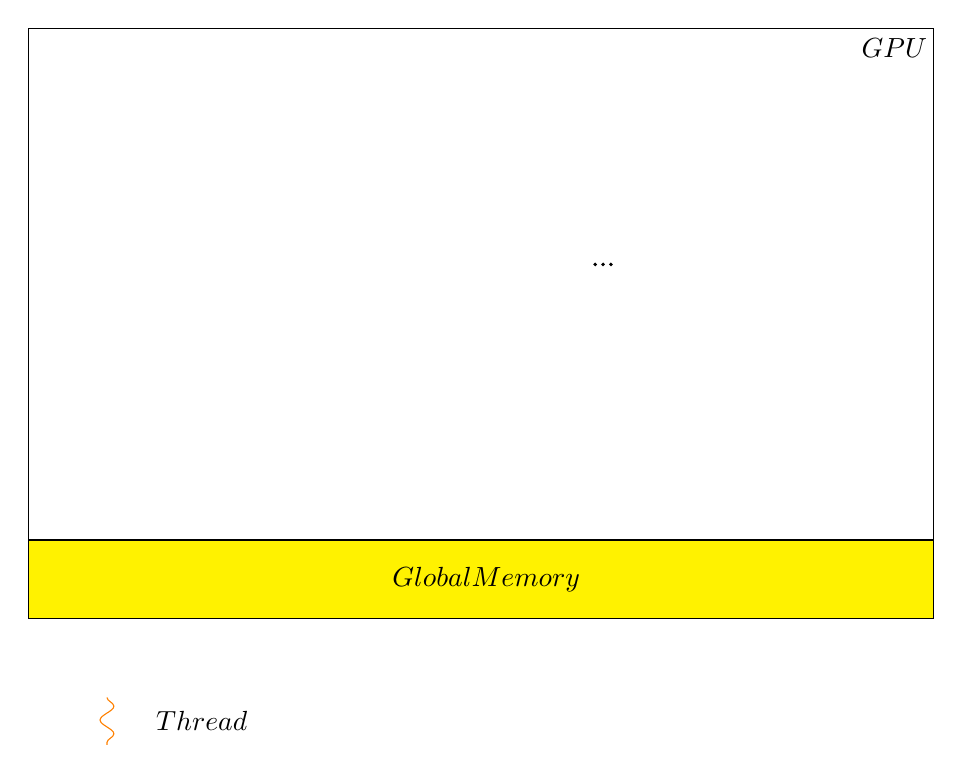
\begin{tikzpicture}
			
			\node[rectangle,
			draw = black,
			text = black,
			anchor = center,
			align=center,
			minimum width = 11.5cm, 
			minimum height = 7.5cm] (cpu1) at (3.75 cm, -0.75cm) {};
			\node[anchor=center] at (9 cm, 2.75 cm) {$GPU$};
			
			%\node[rectangle,
			%draw = black,
			%text = black,
			%anchor = center,
			%align=center,
			%minimum width = 11.5cm, 
			%minimum height = 1.5cm] (cpu1) at (3.75 cm, -6cm) {};
			%\node[anchor=center] at (9 cm, -5.5 cm) {$CPU$};
			
			
			\block{0}{0}{0}
			\block{3.2}{0}{1}
			\block{7.4}{0}{n}
			
			% Dots
			\node  at (5.2cm,0cm) [circle, fill, inner sep=0.5pt] {};
			\node  at (5.3cm,0cm) [circle, fill, inner sep=0.5pt] {};
			\node  at (5.4cm,0cm) [circle, fill, inner sep=0.5pt] {};
			
			
			\node[rectangle,
			draw = black,
			text = black,
			anchor = center,
			fill = yellow,
			align=center,
			minimum width = 11.5cm, 
			minimum height = 1cm] (cpu1) at (3.75 cm,-4cm) {};
			\node[anchor=west] at (2.5 cm, -4 cm) {$Global Memory$};
			
			\draw[orange, snake it] (-1 cm, -5.5cm) to
			(-1 cm, -6.1cm);
			
			\node[anchor=west] at (-0.5cm, -5.8) {$Thread$};
			
		\end{tikzpicture}
	\end{center}
\end{figure}

\subsubsection{Asynchronous Operations} \label{sec:async}

There are two types of engines that can be used to execute kernels in CUDA streams: copy engines and kernel engines. Copy engines are used to copy data between host and device memory, and between different types of memory on the device. Kernel engines are used to execute CUDA kernels. The number of individual engines depends on the actual hardware, lower end GPUs usually have a single kernel and a copy engine, more advanced architectures can have more than one copy or kernel engine.

A CUDA stream is a sequence of commands that are executed in order on a CUDA device. Streams can be used to improve the runtime of a CUDA program by overlapping the execution of different kernels. For example, a copy kernel can be executed in one stream while a compute kernel is executed in another stream. This overlap can lead to a significant performance improvement.


\subsubsection{Synchronization}

Whilst threads within a block can be synchronized, this is not the case for the blocks launched from a kernel. The only real synchronization technique, is to wait for a kernel, meaning all blocks associated with this kernel, to finish and execute a consecutive task using another kernel. 

Since the GPU is limited in its computing and also memory capabilities, the number of blocks which are run in parallel are limited, therefore CUDA cannot give us any guarantee, weather a set of blocks are run serially or in parallel. Some of the blocks might be run in parallel, meanwhile others are run serially. This very constraint, forces the programmer to rethink algorithms and think of ways, how individual subproblems can be run somewhat independently of each other. 

There exists however a way to communicate between blocks in a safe way. Atomic operations can be performed on global memory without any race conditions.

\subsection{Streams}

As described in section \ref{sec:async}, we can leverage streams to improve the runtime a CUDA accelerated application. The way we make use of streams is simple, each thread performs all its computations using on a unique stream. Since leveraging streams only improves the runtime in low numbers because the actual copy and kernel engines are not very numerous, this variant is very simple and effective. We have observed that using more streams on the individual threads does not improve the runtime, quiet contrary it can have a negative impact. 


\subsection{Memory Management}

We use several strategies in order to improve the performance of memory allocation: 

\begin{enumerate}
	\item \textbf{Pinned Memory} As the GPU cannot access the default paged memory directly, when copying memory from the host to the device, the memory must first be copied to pinned memory. This means if we use pinned memory directly with $cudaMallocHost()$, data transfers can be around twice as fast. In our implementation we use pinned memory for all data, which need to be either sent from the host to device or vice versa.
	\item \textbf{Reuse Memory} We can avoid allocation and freeing commands altogether and instead reuse previously allocated memory whenever possible. In our implementation we allocate the memory in the very beginning. Since we have a fixed number of particles as well as an upper limit for the number of cells memory can be allocated when calling the initialize service. The concept is applied to both CPU and GPU memory.
\end{enumerate}

\subsection{GPU Accelerated Count Left}


We have described a CPU implementation of the Count Left Service. In this section we explain how we can port this problem to the GPU. In essence we can use a general reduction as a basis version, and adapt it to sum up up elements which fulfill a certain condition, where the condition is being smaller than a given value. The code is based on the reduction as its explained in a Webinar from \textit{NVIDIA}. \cite{reduction}

\subsubsection{Schedule}

The entire schedule of the GPU accelerated ORB is depicted in figure \ref{fig:orbgpup}. In a first step we call the initialize service, where the necessary data is allocated on all devices and the particles are loaded. Furthermore the initial SPTDS is constructed, which essentially only consists of the root node, encompassing the entire domain and all the particles. Next we enter the main loop of ORB, which iterates until a SPTDS with the desired size is constructed. Within the loop the Count Service is called, computing the number of cells for each cell summed over all the threads in the system. To prepare the data for the GPU transfer a temporary array is made, using the make axis service, which is then sent to the GPU. 
At this stage the actual bisection methods starts on the master, where counting the number of particles left of a cut plane is done with the GPU Count Left service. Depending on the outcome, the cut position is improved respectively and the process is repeated until a nearly perfect cut is found for all the leaf cells of the current SPTDS. For each leaf cell cell two new child cells can be generated using the computed cut positions. Finally the SPTDS can be enriched with the new cell data and the particles array is partitioned accordingly using the Partition service. 
The tree building loop is then repeated or if the desired size of the SPTDS is reached, we exit the loop and call the Finalize service to free the allocated memory.


\begin{figure}[H]
	\begin{center}
		\begin{tikzpicture}
			
			\timeline{6}{14}{3}
			
			
			\parallelloop{-2}{12.5}{8}{1.5}{loop till tree built};
			
			\parallelloop{-1}{9.5}{7}{5.5}{loop till cut found};
			
			\communication{Init}{0}{7}{13};
			
			\communication{Count}{0}{7}{12};
			
			\communication{Make Axis}{0}{7}{11};
			
			\communication{Copy Particles To GPU}{0}{7}{10};
			
			\communication{Count Left GPU}{0}{7}{9};
			
			\process{improve \\ cut}{0}{8};
			
			
			\process{generate\\ new \\ cells}{0}{5};
						
			\communication{Partition}{0}{7}{2};
			
			\communication{Finalize}{0}{7}{1};
			
			
		\end{tikzpicture}
	\end{center}
	\caption{Parallelized ORB GPU version}
	\label{fig:orbgpup}
\end{figure}

\subsubsection{Service}

The GPU version of the Count Left Service invokes the reduction kernel exactly once for every leaf cell of the current SPTDS. Meaning on level 0 of the tree there is only one kernel per processor being executed, when proceeding to further levels, the number of kernels is equivalent to $2^{depth}$ per processor. 
The number of blocks per cell can be determined by $N_{cell}$ divided by the number of threads per block and divided by the number of elements per thread, which is a strategy to increase the thread occupancy. 

All the relevant information can be passed along with the cell can be passed using pass by value  parameters, there is no need to copy any additional data from the CPU to the GPU in advance. The only relevant data is already in global memory, when the particles where copied from the host to the device. Hpwever the results, which are also stored in global memory, need to be copied back from the GPU to the GPU after the kernel has finished.

\subsubsection{Kernel Code}\label{sec:countleftcode}
The actual kernel code is depicted in listing \ref{cuda:reduction}. The input parameters of the reduction kernel (line 13-16) are in order: the input data, which is in sequential order the particles, the output array, where the results of the kernel is stored, the position of the cut plane and finally the total number of elements contained within the cell. Note that since we make use of the Make Axis Service, there is no need to know to which axis the orthogonal cut plane is searched for. 

In a first step on lines 18-20 each thread ID $tid$ is associated with an index in the global memory of input data. Furthermore on line 22-23 the shared data is initialized and set to zero. Its size is equivalent to the block size, the total number of thread per block. Meaning we can store a single float per thread. On lines 25-28 the thread iterates over all elements which it is associated to and copies the results of a compare to shared memory. This allows us to work exclusively with shared memory instead of global memory, reducing the amount of costly memory accesses.

There exists an optimum in terms of number of operation performed by a single thread. In order to adapt the number of ops dynamically, the while loop ensures that each thread iterates over a certain number of elements as seen in lines 25-28. The input parameter $n$ defines the total number of particles. Therefore if we reduce the total number of blocks by a factor of $r$, the while loop will iterate over $r$ elements. Inside the while loop on line 27 the index $i$ is incremented by $gridSize$ in each iteration. The grid size is equivalent to the total number of threads associated with the kernel. Therefore when launching the kernel, the number of blocks can be divided by $r$ which then results in $r$ iterations performed in the while loop. In our case we set $r$ to 16 as more or less items per thread will result in a lower performance.

The rest of the kernel code performs the actual reduction, where in each step two elements from the shared memory are summed together. Given a block size of 256, after line 37 exactly 256 sums are stored in shared memory. In a next step as seen on line 37 (lines 31-36 are not relevant as the size is smaller than 512) the left half threads in the block add their value together with the values stored in a position offset by 128. This step reduces the total number of elements to be considered to 128, and the step can be repeated as seen on lines 42 to 46. 

The reduction is optimized by using a template, which indicates the total number of thread per block, which is equivalent to the blockSize. Since the template is evaluated at compile time, all the if statements taking blockSize as a parameter in figure do not cause any performance loss. In fact, because  the reduction loops are unrolled (31-52) the the performance of the kernel is increased. 

Each time there is a control statement involving non template arguments, a branch divergence is introduced. On the GPU these divergences become problematic bad when they are introduced inside a warp. Meaning if any of the 32 within a warp execute a different code from the other threads, the warp cannot function optimally anymore. For this reason, the $warpReduce$ method as seen on line 2-9 is introduced. This method is only executed when there are 64 elements in shared memory which are still to be summed, which requires only 32 threads as every thread in each iteration sums two elements together. Inside the warp reduce method, there are more unrolled loops continuing the same patterns as described above. However in this case there are no control statements that could introduce a warp divergence, which means there are computations performed which are not actually necessary, however as the computations inside a warp are executed in parallel anyways, this comes with no performance penalties. Inside a warp there is no need for synchronization as all threads are executed in parallel. 

\begin{lstlisting}[language=c++, caption=Conditional Reduction in CUDA, label=cuda:reduction]
template <unsigned int blockSize>
extern __device__ void warpReduce(
	volatile int *sdata, unsigned int tid) {
	if (blockSize >= 64) sdata[tid] += sdata[tid + 32];
	if (blockSize >= 32) sdata[tid] += sdata[tid + 16];
	if (blockSize >= 16) sdata[tid] += sdata[tid + 8];
	if (blockSize >= 8) sdata[tid] += sdata[tid + 4];
	if (blockSize >= 4) sdata[tid] += sdata[tid + 2];
	if (blockSize >= 2) sdata[tid] += sdata[tid + 1];
}

template <unsigned int blockSize>
extern __global__ void reduce(
	float *g_idata,
	 unsigned int*g_odata, 
	 float cut, 
	 int n) {
	unsigned int tid = threadIdx.x;
	unsigned int i = blockIdx.x*(blockSize) + threadIdx.x;
	unsigned int gridSize = blockSize*gridDim.x;
	
	__shared__ int sdata[blockSize];
	sdata[tid] = 0;
	
	while (i < n) {
		sdata[tid] += (g_idata[i] <= cut);
		i += gridSize;
	}
	__syncthreads();
	
	if (blockSize >= 512) {
		if (tid < 256) {
			sdata[tid] += sdata[tid + 256];
		}
		__syncthreads();
	}
	if (blockSize >= 256) {
		if (tid < 128) {
			sdata[tid] += sdata[tid + 128];
		} __syncthreads();
	}
	if (blockSize >= 128) {
		if (tid < 64) {
			sdata[tid] += sdata[tid + 64];
		} __syncthreads();
	}
	if (tid < 32) {
		warpReduce<blockSize>(sdata, tid);
	}
	if (tid == 0) {
		g_odata[blockIdx.x] = sdata[0];
	}
}
\end{lstlisting}



Initializing the kernel once for each cell is a simple solution, however as we increase the number of cells, more and more calls to the kernel are made. Calls are not free of cost, as there is some overhead with each initialization of a kernel. Thus the performance degrades gradually as the tree is built, because on each level the number of cells for which the bisection method is executed doubles. At some point, the overhead even dominates over the actual computations by a lot. 


\subsection{Improved GPU Accelerated Count Left} \label{imprctl}

To solve the degrading performance problem we make some changes to the kernel and the overall schedule. The main idea is to prepare the necessary data for all cells in advance, effectively reducing the overall number of necessary kernel calls to $\lceil \log_2 d \rceil $ instead of $2 \times d$. In figure \ref{fig:degrading} the resulting number of kernel calls are compared for both versions. Each block is provided with information concerning the start and end index of the cells particles, the cut position as well as an index of the cell. 


\begin{figure}[H]
	\begin{center}
		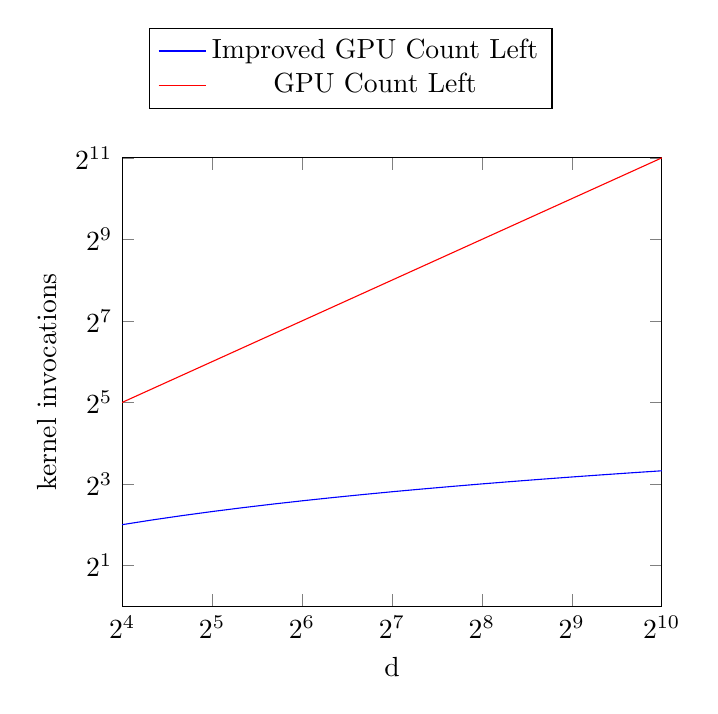
\begin{tikzpicture}
			\begin{axis}[
				xmode=log,
				ymode=log,
				log basis x={2},
				log basis y={2},
				xlabel={d},
				ylabel={kernel invocations},
				%x filter/.code=\pgfmathparse{#1 + 6.90775527898214},
				xmin = 16, xmax = 1024, ymin= 1, ymax=2048,
				legend style={at={(0.05,1.2)},anchor=west}]
				
				
				\addplot+[name path = A, domain = 16:4096, mark=none] {
					ln(\x) / ln(2) 
				};
				
				\addlegendentryexpanded{Improved GPU Count Left};
				
				\addplot+[name path = A, domain = 1:4096, mark=none] {
					2 * \x 
				};	
				
				\addlegendentryexpanded{GPU Count Left};
				
				
			\end{axis}
		\end{tikzpicture}
		\caption{Kernel calls with GPU count left versions}
		\label{fig:degrading}
	\end{center}
\end{figure}

We will explain the improved version using a simple example: Let us consider $cell_2$ with a volume that encompasses particles in the range 0 - 10240. $cell_3$ encompasses particles in the range 10240 - 20480. We have a blocksize of 256 threads and the elements per thread are 16, thus each block processes $256 * 16 = 4096$ elements. In this case we reserve three blocks for each cell, where the first block processes elements 0 - 4096 and the second one 4096 - 10240. By assigning more work to the second block, we make sure that there are no underworked threads, as measurements have shown a slight increase in elements per thread is better than a decrease. Furthermore we can avoid blocks where not even all the threads are occupied, because less than 256 elements are processed on the block. Consequently the third and fourth block respectively process particles 10240 to 14446 and 14446 to 20480. Since the number of required blocks for cell is known as well as the exact range of particles for which the reduction has to be computed, we can copy all this information to the GPU in advance and simply launch a kernel with the total block sum. 
Each kernel stores its information in an output array where the assignment between the output and the actual cell is known. The service therefore needs to iterate over all the output which have been computed by the blocks associated with a kernel and output them at a single cell specific location in the output $ou$ array of the service.

\subsubsection{Schedule}

Only a single change is made to the schedule: We introduce another service which is called GPU Copy Cell Service, which does as the name says, copying the cell information from the CPU to the GPU. Since only the cut positions change while we are iterating over the inner loop, this service can be called outside of it. The Improved GPU Count Left Service copies the cut data each time it is invoked. Other than that, the schedule remains equal. 

\begin{figure}[H]
	\begin{center}
		\begin{tikzpicture}
			
			\timeline{6}{15}{3}
			
			
			\parallelloop{-2}{13.5}{8}{1.5}{loop till tree built};
			
			\parallelloop{-1}{9.5}{7}{5.5}{loop till cut found};
			
			\communication{Init}{0}{7}{14};
			
			\communication{Count}{0}{7}{13};
			
			\communication{Make Axis}{0}{7}{12};
			
			\communication{Copy Particles To GPU}{0}{7}{11};
			
			\communication{Copy Cells To GPU}{0}{7}{10};
			
			\communication{Improved Count Left GPU}{0}{7}{9};
			
			\process{improve \\ cut}{0}{8};
			
			
			\communication{Partition}{0}{7}{5};
			
			\communication{Finalize}{0}{7}{1};
			
			\process{generate\\ new \\ cells}{0}{4};
			
		\end{tikzpicture}
	\end{center}
	\caption{Parallelized ORB GPU version 2}
	\label{fig:orbgpup2}
\end{figure}


\subsubsection{Kernel Code}

The kernel code as seen in listing \ref{ctlocuda} largely remains the same. New data pointers are passed along as a parameter where $g_begin$ and $g_end$ mark the begin and end of the important particle array slice, furthermore $g_cuts$ is an array of cell cuts for each block. As we prepare the data in a way, that each block only needs to operate over the particles contained within a single cell, the data can be read using the blockIdx.x (lines 20 - 22) which is a CUDA variable and provides a sequential indexing of blocks associated with the kernel. Everything else, including the subroutine $warpReduce$ remain equal. 

\begin{figure}[H]
	\begin{lstlisting}[language=c++, caption=Kernel Optimized GPU Count Left, label = ctlocuda]
template <unsigned int blockSize>
extern __global__ void reduce(
float * g_idata,
unsigned int * g_begins,
unsigned int * g_ends,
float * g_cuts,
unsigned int * g_odata) {
	__shared__ unsigned int s_data[blockSize];
	
	unsigned int tid = threadIdx.x;
	const unsigned int begin = g_begins[blockIdx.x];
	const unsigned int end = g_ends[blockIdx.x];
	const float cut = g_cuts[blockIdx.x];
	
	unsigned int i = begin + tid;
	s_data[tid] = 0;
	
	// unaligned coalesced g memory access
	while (i < end) {
		s_data[tid] += (g_idata[i] <= cut);
		i += blockSize;
	}
	__syncthreads();
	
	if (blockSize >= 512) {
		if (tid < 256) {
			s_data[tid] += s_data[tid + 256];
		}
		__syncthreads();
	}
	if (blockSize >= 256) {
		if (tid < 128) {
			s_data[tid] += s_data[tid + 128];
		} __syncthreads();
	}
	if (blockSize >= 128) {
		if (tid < 64) {
			s_data[tid] += s_data[tid + 64];
		} __syncthreads();
	}
	if (tid < 32) {
		warpReduce<blockSize>(s_data, tid);
	}
	if (tid == 0) {
		g_odata[blockIdx.x] = s_data[0];
	}
}
	\end{lstlisting}
	\caption{Reduction in CUDA}
	\label{cuda:reduction2}
\end{figure}

\subsection{GPU Accelerated Partitioning}

We have successfully implemented a version with a GPU accelerated Count Left. Since the particles are still partitioned on the CPU, the data needs to be copied to GPU each time we expand the SPTDS. As we use the Make Axis service to compress the axes into a single array, we only need to copy $N$ elements, but we need to do so $\lceil \log_2 d \rceil$ times. 
If we partition the particles on the GPU, the data needs to be copied only once, but in this case all three coordinates have to be copied, thus $
N \times 3$. Nevertheless this corresponds a fraction of the total data transfer: $\frac{3}{\lceil \log_2 d \rceil \times}$. In figure \ref{fig:transfer} its observable that a GPU partition becomes feasible, at least in terms of data transfer, after $d$ exceeds 16. 

\begin{figure}[H]
	\begin{center}
		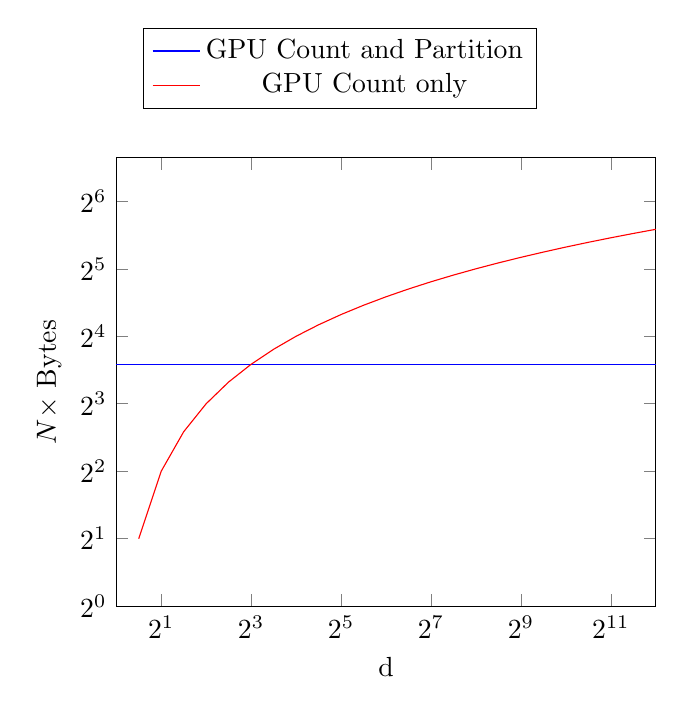
\begin{tikzpicture}
			\begin{axis}[
				xmode=log,
				ymode=log,
				log basis x={2},
				log basis y={2},
				xlabel={d},
				ylabel={$N \times$ Bytes},
				%x filter/.code=\pgfmathparse{#1 + 6.90775527898214},
				xmin = 1, xmax = 4096, ymin= 1, ymax=100,
				legend style={at={(0.05,1.2)},anchor=west}]
				

				\addplot+[name path = A, domain = 1:4096, mark=none] {
					3 * 4
				};
			
				\addlegendentryexpanded{GPU Count and Partition};
			
				\addplot+[name path = A, domain = 1:4096, mark=none] {
					ln(\x) / ln(2) * 4
				};	
				
				\addlegendentryexpanded{GPU Count only};

				
			\end{axis}
		\end{tikzpicture}
		\caption{Data transferred with and without GPU partitioning}
		\label{fig:transfer}
	\end{center}
\end{figure}


A GPU partitioning algorithm was first proposed by Cederman \cite{GPUQ} and later refined by Manca \cite{CUDAQ} where atomic operations are leveraged to improve the runtime of the algorithm. Our version is built around the concepts introduced by Manca. 

Early results have shown partitioning the data on the GPU is not really faster than the CPU version where the CPU version is not even implemented in a optimal manner and finally the number of particles which can be stored on the GPU memory is reduced by $\frac{5}{3}$. This is caused by required additional temporary arrays for memory swaps on the GPU. Furthermore there was not enough time to fully optimize and track down all issues with the code, therefore we do not describe the full kernel code and instead limit ourselves to introduce the ideas for subsequent work. 

\subsubsection{Schedule}

In the adapted schedule (figure \ref{fig:orbgpu3}) we can move the Copy Particles To GPU service out of the main loop, other than that the schedule remains the same. 

\begin{figure}[H]
	\begin{center}
		\begin{tikzpicture}
			
			\timeline{6}{14}{3}
			
			
			\parallelloop{-2}{11.5}{8}{1.5}{loop till tree built};
			
			\parallelloop{-1}{9.5}{7}{5.5}{loop till cut found};
			
			\communication{Init}{0}{7}{13};
			
			\communication{Copy Particles To GPU}{0}{7}{12};
			
			\communication{Count}{0}{7}{11};
		
			
			\communication{Copy Cells To GPU}{0}{7}{10};
			
			\communication{Count Left GPU}{0}{7}{9};
			
			\process{improve \\ cut}{0}{8};
			
			
			\communication{Partition}{0}{7}{5};
			
			\communication{Finalize}{0}{7}{1};
			
			\process{generate\\ new \\ cells}{0}{4};
			
		\end{tikzpicture}
	\end{center}
	\caption{Parallelized ORB with GPU counting and GPU partitioning}
	\label{fig:orbgpu3}
\end{figure}


\subsubsection{Partitioning a Single Cell}

In a first step we perform a block wise partition, meaning there is no synchronization between blocks at this stage. Each thread loads the particle coordinate of the matching axis into the shared memory register $S$. We then make two copies of the data stored in the shared memory, the first copy $A$ compares each value with the cut and stores 0 if the value is smaller and 1 otherwise. The second copy $B$ stores the inverted result. 
We now perform a parallel prefix sum, or scan, on both copies. We can use an algorithm as it is described in GPU Gems \cite{SCAN}. On $B$ we add the total number of elements smaller than the cut to each element. 
In theory the block wise partition could already be applied by storing each element with index $i$ larger than the cut at $A_i$ and larger elements at $B_i$. 
However our goal is to partition all elements across multiple blocks. To do so we introduce a global variable called $leq$ and $g$ where the total number of elements smaller equal and bigger than the cut are stored. Each time a block has computed both scans, the number of elements designated to the block smaller and larger than the cut are known. Thus a single thread of each block performs an atomic add on $leq$ and $g$ accordingly. $AtomicAdd()$ returns the old value of the variable. Therefore we can use and store it in two designated shared memory register $s_leq$ and $s_g$. 
At this stage every thread in a block agrees on a value for $s_leq$ and $s_g$ the values can be treated as starting indices to store the block wise partitioned results in the output array. In this case however we store an element larger than the cut at position $i$ in location $A_i + s_leq$ and otherwise at $B_i = s_g$. 

In our case the input array are coordinate values of particles and the output array is a temporary array of size $N$. The in an output array cannot be the same as the partition cannot be performed in place. Doing so would result in elements that are overwritten before they are read by the thread assigned to it. This cannot be avoided with the proposed technique as the relationship between the range of input data treated by a kernel and the output is not deterministic. Its dictated by the order, by which the kernel reach the $atomicAdd()$ statement. 

As of now only a single axis is partitioned, but the same needs to be done for the other two axes. One approach is to partition all the other arrays in the same kernel, as the permutations can simply be reapplied. However in this case we need three additional temporary arrays, one for each axis. Further Reducing the number of particles which can be stored on the GPU by $\frac{1}{2}$. A more memory efficent, but slightly slower variant is to allocate another array on the GPU where the actual permutation indices are stored when the partition kernel is executed. Therefore together with the temporary array $N$ is only reduced by $\frac{3}{5}$. After the partition kernel has finished, we can copy back the coordinates from the temporary array to the original location in a device to device copy. Then the second axis is partitioned using the precomputed permutations and the results are again copied back to the proper location. Finally after the step is repeated for the last axis, the partition is finished.

\subsubsection{Partitioning Multiple Cells}

We apply the same method as introduced in section \ref{imprctl} to ensure only a single kernel has to be launched for all cells. 
Each block is assigned a cell, where all relevant information about the cell is stored in different arrays in global memory. Each block then read the designated data by acessing the arrays at index $blockIdx.x$. The variables $leq$ and $g$ are replaced by arrays of the same length as there are cells to be partitioned (which is not equivalent to the number of blocks). This ensures all the blocks assigned to a single cell perform the atomic operations on the same variable. For a block to know which element in the $leq$ and $g$ arrays it needs to access, a sequential cell index array is passed, where all blocks working on the same cell receive the same cell index. 


\newpage
\section{Performance Analysis of ORB}\label{sec:empan}

All measurements where performed on Piz Daint where the performance of system can be read from table \ref{fig:datapoints}. The supercomputer uses a slurm workload manager. \cite{Slurm} Simple job script can be executed using $sbatch$. In our case we used a meta script which has the function of modifying the actual job scripts for the desired parameters. 


\begin{figure}[H]
	\begin{center}
		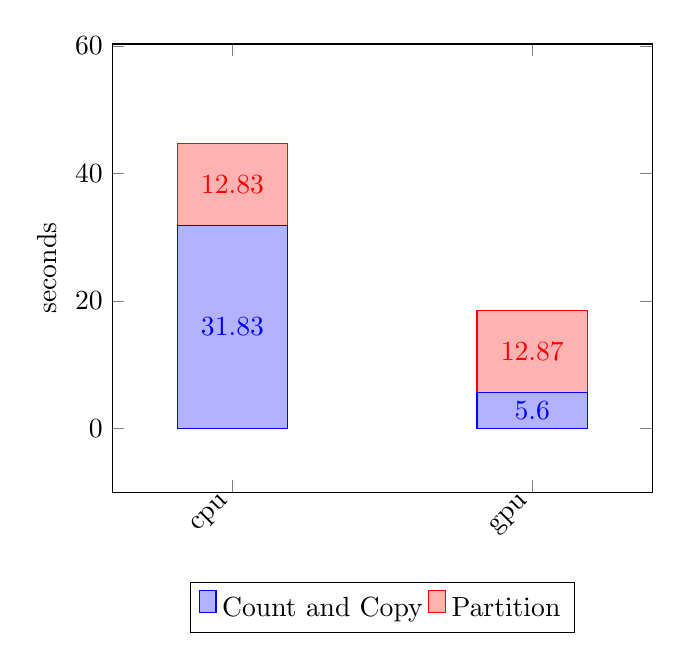
\begin{tikzpicture}
			
			\begin{axis}
				[
				 enlargelimits=0.4,
				ybar stacked,
				bar width=40pt,
				nodes near coords,
				legend style={at={(0.5,-0.20)},
					anchor=north,legend columns=-1},
				ylabel={seconds},
				symbolic x coords={cpu, gpu},
				xtick=data,
				x tick label style={rotate=45,anchor=east}]
				ymin=0,
				ymax=50
				]
				\addplot+[ybar] plot coordinates {(cpu, 31.83) (gpu, 5.60)};
				\addplot+[ybar] plot coordinates {(cpu, 12.83) (gpu, 12.87)};

			\legend{\strut Count and Copy, \strut Partition}
			\end{axis}
			
			
		\end{tikzpicture}
	\end{center}
	
	\caption{Execution times of different strategies}
	\label{fig:analy2}
\end{figure}

In figure \ref{fig:analy2} the final measurements are plotted. The total runtime of the ORB is around 43 seconds when performed only on the CPU, for the GPU accelerated version it comes down to 18 seconds. However a large part of the execution time can be attributed to the Partitioning, where its overhead remains equal for both versions. Even the CPU Partitioning can be improved a lot and the GPU version might increase the performance even further. 
If we subtract the time lost for the partitioning, the GPU version is about $5.6$ times faster, which even slightly worse than the expected speedup of $6.2$. The difference can mostly be explained by additional overheads, especially as the GPU kernel has to touch the elements more than once due to the way the reduction was implemented. 

When we look at the absolute number there is a stark difference: $56.47s$ predicted for the CPU version were $31.83$ was the actual timing. Similarly the GPU was expected to execute ORB (without the partitioning) in $8.99s$, however it only took $5.6s$. The theoretical model considers an upper bound for the total number of iterations which the bisection method takes to converge. In reality this number is closer to 20 than to $p$ which is 32 in the measured data. When considering this, the measurements are also in an absolute term relatively close to the theoretical model. $56.47s \times \frac{20}{32} = 37s$ against the actual $31.83s$ and $8.99s \times \frac{20}{32} =5.99s$ compared to $5.6s$.
\subsection{Scaling}

To make sure the GPU version scales good we have evaluated the total runtimes for 


\begin{filecontents*}{results0.csv}
	p, d, t, t2
	1048576, 10, 0.04
	4194304, 10, 0.14
	16777216, 10, 0.61
	67108864, 10, 2.57
	268435456, 10, 11.15
	1073741824, 10, 47.58, 
\end{filecontents*}

\begin{filecontents*}{results1.csv}
	p, d, t, t2
	1048576 , 10, 0.04
	4194304, 10, 0.10
	16777216 , 10, 0.33
	67108864 , 10, 1.24
	268435456 , 10, 4.98
	1073741824, 10, 20.31
\end{filecontents*}

\begin{figure}[H]
	\begin{center}
		\begin{tikzpicture}
			
			\begin{axis}
				[
				xlabel={number of particles},
				ylabel={seconds},
				nodes near coords,
				xmin=1048576,
				xmax=1073741824,
				ymin=0,
				ymax=64,
				xmode=log,
				ymode=log,
				log basis x={2},
				log basis y={2},
				legend style={at={(1.05,0.6)},anchor=west}]
				]
				\addplot+[
				point meta=explicit symbolic
				] table [
				x=p, 
				y=t, 
				col sep=comma] 
				{results0.csv};
				\addlegendentryexpanded{CPU Only};
				\addplot+[
				point meta=explicit symbolic
				] table [
				x=p, 
				y=t, 
				col sep=comma] 
				{results1.csv};
				\addlegendentryexpanded{GPU Count Left};
			\end{axis}
			
			
		\end{tikzpicture}
	\end{center}
	
	\caption{Execution times of different strategies}
	\label{fig:analy}
\end{figure}

\newpage
\section{Conclusion}


% Use for reduction explanation https://texample.net/tikz/examples/database-decimation-process/
\bibliographystyle{unsrt}
\bibliography{reference}

\listoffigures
\listoftables

\end{document}
